% replace default bibliography style
\RequirePackage{etoolbox}
\patchcmd{\bibliographystyle}{#1}{unsrtnat}{}{}


\documentclass[fleqn,10pt]{wlscirep} 
\usepackage{array,longtable,multirow}
\usepackage{fancyhdr}
\geometry{a4paper}

\usepackage[tableposition=below]{caption}
\captionsetup[longtable]{skip=1em}

\pagestyle{fancy}
\fancyhf{}
\lfoot{© 2018 by the Authors}
\rfoot{Page \thepage}
\cfoot{FIM4R Version 2.0}

\usepackage[sort&compress,square,numbers,longnamesfirst]{natbib}

\title{Federated Identity Management for Research Collaborations}
\date{\today}

\usepackage {authblk}
\renewcommand\Authands{ and }
\renewcommand\Affilfont{\normalfont\small}


\makeatletter
\renewcommand\AB@affilsepx{; \protect\Affilfont}
\makeatother

\author[8]{C~J~Atherton}
\author[27]{T~Barton}
\author[17]{J~Basney}
\author[16]{D~Broeder}
\author[10]{A~Costa}
\author[23]{M~van~Daalen}
\author[15]{S~O~M~Dyke}
\author[2]{W~Elbers}
\author[5]{C-F~Enell}
\author[11]{E~M~V~Fasanelli}
\author[6]{J~Fernandes} 
\author[8]{L~Florio}
\author[4]{P~Gietz}
\author[20]{D~L~Groep}
\author[11]{M~Junker}
\author[8]{C~Kanellopoulos}
\author[25]{D~P~Kelsey}
\author[25,29]{P~J~Kershaw}
\author[10]{C~Knapic}
\author[9]{T~Kollegger}
\author[28]{S~Koranda} 
\author[3]{M~Linden}
\author[7]{F~Marinic}
\author[14]{L~Matyska}
\author[3]{T~H~Nyrönen}
\author[12]{S~Paetow} 
\author[22]{L~Paglione}
\author[11]{S~Parlati}
\author[30]{C~Phillips}
\author[1,14]{M~Prochazka}
\author[24]{N~Rees}
\author[6]{H~Short}
\author[13]{U~Stevanovic}
\author[18]{M~Tartakovsky} 
\author[26]{G~Venekamp}
\author[30]{T~Vitez}
\author[6]{R~Wartel}
\author[18]{C~Whalen}
\author[19]{J~White}
\author[21]{C~Zwolf}


\affil[1]{CESNET, Prague, Czech Republic}
\affil[2]{CLARIN ERIC, Utrecht, The Netherlands}
\affil[3]{CSC -- IT Center for Science, ESPOO, Finland}
\affil[4]{DAASI International, Tübingen, Germany}
\affil[5]{EISCAT Scientific Association, Kiruna, Sweden}
\affil[6]{European Organization for Nuclear Research (CERN), Geneva, Switzerland}
\affil[7]{European Space Agency (ESA/ESAC), Madrid, Spain}
\affil[8]{GÉANT Association, Amsterdam, The Netherlands}
\affil[9]{GSI Helmholtzzentrum für Schwerionenforschung, Darmstadt, Germany}
\affil[10]{INAF- National Institute for Astrophysics - Italy}
\affil[11]{INFN - National Institute for Nuclear Physics - Italy}
\affil[12]{Jisc, Harwell, United Kingdom}
\affil[13]{Karlsruhe Institute of Technology (KIT), Karlsruhe, Germany}
\affil[14]{Masaryk University (MU), Institute of Computer Science (ICS), Brno, Czech Republic}
\affil[15]{McGill University, Montreal, Canada}
\affil[16]{Meertens Institute, Amsterdam, The Netherlands}
\affil[17]{National Center for Supercomputing Applications, University of Illinois, Urbana-Champaign, USA}
\affil[18]{National Institute of Allergy and Infectious Diseases, Rockville, Maryland USA}
\affil[19]{NeIC, Oslo, Norway}
\affil[20]{Nikhef, Amsterdam, The Netherlands}
\affil[21]{Observatoire de Paris (Obspm), France}
\affil[22]{ORCID Inc, Bethesda, Maryland USA}
\affil[23]{Paul Scherrer Institute, 5232 Villigen PSI, Switzerland}
\affil[24]{SKA Organisation, Jodrell Bank, Lower Withington, Macclesfield, United Kingdom}
\affil[25]{STFC UK Research and Innovation, Rutherford Appleton Laboratory, Didcot, United Kingdom}
\affil[26]{SURFsara, Amsterdam, The Netherlands}
\affil[27]{University of Chicago, Chicago, Illinois, USA}
\affil[28]{University of Wisconsin-Milwaukee (UWM), Milwaukee, Wisconsin USA}
\affil[29]{NCEO (National Centre for Earth Observation), NERC, United Kingdom}
\affil[30]{Canarie, Ottawa, Canada}

 
 
 
 
 




\begin{abstract}
This white-paper expresses common requirements of Research Communities seeking to leverage Identity Federation for Authentication and Authorisation. Recommendations are made to Stakeholders to guide the future evolution of Federated Identity Management in a direction that better satisfies research use cases. The authors represent research communities, Research Services, Infrastructures, Identity Federations and Interfederations, with a joint motivation to ease collaboration for distributed researchers. The content has been edited collaboratively by the Federated Identity Management for Research (FIM4R) Community, with input sought at conferences and meetings in Europe, Asia and North America. 
\end{abstract}

\begin{document}

\flushbottom


\maketitle

\thispagestyle{empty}

\noindent \\ \\ \\ \\ {\textbf{E-mail: contact@fim4r.org} \\  \\ For the ORCID{\textsuperscript{\textregistered}} identifiers and author affiliations of the ``Federated Identity Management for Research" collaboration to their various Research Communities and e-Infrastructures, see Appendix \ref{Authors}.
\newline
\newline
\noindent {\textbf{Document details} - Version: 2.0.  Date: 3 July 2018 \\ doi: 10.5281/zenodo.1296032 }
\newline

\vfill

\noindent © 2018 by the Authors. This work is licensed under a Creative Commons Attribution 4.0 International License. To view a copy of this license, visit http://creativecommons.org/licenses/by/4.0/ or send a letter to Creative Commons, PO Box 1866, Mountain View, CA 94042, USA.

\newpage
\tableofcontents
\newpage
\section{Introduction}
``Federated identity management (FIM) is an arrangement that can be made among multiple organisations that lets subscribers use the same identification data to obtain access to the secured resources of all organisations in the group. Identity federation offers economic advantages, as well as convenience, to organisations and their users. For example, multiple institutions can share a single community application, with resultant cost savings and consolidation of resources. In order for FIM to be effective, the partners must have a sense of mutual trust."\cite{FIM4Rv1:2012}\footnote{For any particular organisation the term ``resources" may refer to any combination of data, compute services, and research instruments.} 

Many research fields are facing the challenge of a deluge of scientific data that needs to be accessed by expanding user bases in dynamic collaborations that cross organisational and national boundaries. Driven by these needs, representatives from a variety of communities, including photon/neutron facilities, social science \& humanities, high-energy physics, atmospheric science, bioinformatics and fusion energy, came together in 2012 to publish a set of joint requirements. A common vision for FIM across these communities was presented as well as the key stages of a roadmap and a set of recommendations intended to ensure its implementation. 

The initial white-paper proved highly influential in the wider community, with impact seen in the Research and Education Federations Group (REFEDS)\cite{refeds}, the GÉANT Project\cite{GN4}, and in the creation of the EU-funded project on Authentication and Authorisation for Research and Collaboration (AARC)\cite{aarc}. Much progress has been made over the past few years. Several of the original requirements have been addressed whilst others remain open, a subset have been found to be no longer relevant, and additional requirements have been identified that reflect the evolved landscape. 

\subsection{About FIM4R}
FIM4R\cite{fim4rweb} (Federated Identity Management for Research) is a collection of research communities and infrastructures with a shared interest in enabling Federated Identity Management for their research cyber infrastructures. After publishing the initial white-paper in 2012, FIM4R has remained an active community that meets on a biannual basis to exchange ideas, challenges and best practices in FIM.  

\subsection{Vision}
The FIM4R authors envisage this paper to be influential in guiding the development of Federated Identity Management technology and policy in the coming years. It is hoped that the paper will be read widely, by funding agencies, technology providers, policy makers and other stakeholders, and that future progress will reflect the requirements and recommendations of the research communities represented here. This work represents the current challenges and status of research communities and effort has been made to be as technology agnostic as possible. The contributors aspire for this content to remain relevant as the protocols and tools continue to evolve. 

\subsection{Structure of the Paper}
This paper begins with an overview of the current landscape of Federated Identity Management and its evolution since the initial FIM4R paper\cite{FIM4Rv1:2012} in 2012, which we’ll refer to as ``FIM4R v1". It then presents statistics describing the number and distribution of participating researchers and computing centres comprising research communities that participated in contributing to this white paper. Next, a curated list of requirements gathered through discussion among research communities is reported together with some analysis of that data. 

Based on this data and its analysis, recommendations are identified, together with those groups best positioned to address each of them, which provide specific guidance for shaping the future of FIM in line with the needs of research communities. An appendix contains a narrative description of each participating research community. These convey the current status of authentication and authorisation in different disciplines and highlight some of their particular challenges. 

\section{The Evolution of Federated Identity Management}
``Authenticate locally, authorise globally" was the rallying cry of those who originally conceived of what we now call FIM. Its three main aims were to deliver good user experience by extending the reach of campus credentials far beyond where the campus can take them, and simultaneously reduce the number of credentials users need to deal with; to leverage campus credential management practices to produce a dividend for relying parties, who could then focus more of their energy on their services; and, finally, to make federation a global infrastructure so that academic collaboration, itself global, benefits. In a very substantial sense, this has been done. FIM now spans the national R\&E federations from many countries into an aggregated whole known as eduGAIN\cite{edugain}, operated on a sustained basis by GÉANT, that contains thousands of entities operated by thousands of organisations. 

The ``authorise globally" part has proved rather hard. Access policies are built either by listing individual users or by performing a check on their attributes (or attributes of their credential management practices). The value of FIM per se is constrained by the availability of valuable attributes it conveys. The difficulty in identifying the most valuable attributes and the change management to produce them scales directly with FIM’s reach. With thousands of organisations participating in FIM worldwide, these are considerable ongoing challenges, driving much of FIM’s evolution and the reason for several of the recommendations below. 

For a long while, needs and issues like these were conceived only in the context of a singular infrastructure: that operated by the national R\&E federations. Support more users, i.e., support more academic collaborations, by getting more campuses and research collaborations directly enrolled in FIM, and somehow induce each campus to improve its credential management practices to source valuable attributes and keep abreast of best practices, their share of enabling ``authorise globally". 

In response, the conception of FIM gradually began to evolve. Some national R\&E federations centralised the federation operations of their members, reducing the change management problem (though sometimes creating other issues in the process). Social ID gateways admitted users without waiting on their campus to get on board with FIM, the ``long tail" problem of the original conception of FIM. Credential providers for unaffiliated users started to pop up. Research e-Infrastructures experimented with proxies as a more efficient means to extend the value of FIM across an existing system of research services compared to retrofitting each research service to interoperate with federation on its own. These proxies also provided a platform on which to mitigate attribute deficiencies of national R\&E federations and address the long tail problem, at least for their users, sometimes by relying on ORCID\cite{orcid} or other generally-available services as a credential provider. Services specialised in the niche of linking accounts, translating tokens, and other interoperability needs between R\&E federations and research e-Infrastructures, permitting proxies to further specialise in how authorisation is managed. The Research Community Proxy section below explores this key development in greater depth.

Additional federating technologies such as OAuth2/OIDC\cite{oidc} and Moonshot\cite{moonshot} began to be used to address use cases ill-suited to many SAML implementations. And the sheer scale of FIM has begun to bog down the means by which R\&E federation operators have been managing their members’ SAML metadata, prompting a shift in this fundamental process a step in the direction of how it’s proposed to be done for OIDC\cite{oidcfed}. 

Privacy and security concerns have increased along with the technical and organisational evolution of FIM. The EU’s General Data Protection Regulation (GDPR)\cite{GDPR:2016}\cite{eugdpr}, and Facebook in a different way more recently, have motivated many to seriously attend to the privacy characteristics of how user attributes are managed and protected in FIM\cite{assessdp}\cite{attributerelease}\cite{baseline}\cite{dpcoco}. Security sufficient to protect confidentiality of personal data is a key element of privacy, and the ability to respond to a FIM-related security incident has become a critical aspect of FIM operations\cite{sirtfi}. While privacy and security measures are good and necessary in their own right, their implementation fosters trust and confidence in FIM, which in turn reduces inhibition to share limited user attributes and hence increases the overall value of FIM to research. This rationale underlies some of the recommendations below.

FIM is now becoming an ecosystem layered on top of the original aims and this is much richer than that conceived at the outset. FIM now comprises more kinds of technology provided by more types of organisations who layer production quality operations on top of what R\&E federation operators provide. The shift from the original to this evolved conception of FIM is reflected in the requirements gathered from research communities that are reported in the Analysis of Common Requirements section below and in the growing diversity of parties needed to address them.

\subsection{The Research Community Proxy}
As discussed above, eduGAIN and the national R\&E identity federations enable the federation of identities and services at a global scale. Users can use the identities provided by their home institution to access services available to them via their federation and eduGAIN. In this model there is a direct or indirect relationship between the users’ home institution and the service providers facilitated by the national federations and eduGAIN. Although this model is sufficient for users who are doing their everyday work as members of their home institution, it is often insufficient to enable their collaborative research activities with colleagues from other institutions across organisational or national boundaries. The relationship between the users' home institutions and service providers, which is typically found in the national identity federations and eduGAIN, now needs to become a relationship between a research community, the users' home institutions and service providers. In the context of such research collaborations, it is the participation in the collaboration (membership) which constitutes the basis for being able to access and share resources that are available to the members of the collaboration; the membership information is not known to the IdP nor to eduGAIN.  Within a research collaboration also more fine-grained memberships can be specified, e.g. to map roles within a particular service resulting to a research infrastructure wide authorisation system.

Since FIM4R v1 was published in 2012, we have been witnessing more and more research communities implementing Research Community Proxies, which enable the integration of:
\begin{itemize}
  \item user registration and group management systems used by the communities, with 
  \item federated identities coming primarily from the home institutions of the users, but also with other identity sources for users who do not have access to federated users accounts and with 
  \item services providers, which provide access to various types of resources necessary for the research collaboration. 
\end{itemize}

The Research Community Proxy provides a single integration point, on which a research community can integrate its user registration and group management system, community services and federated identity providers. The Research Community Proxy is responsible for dealing with the complexity of integrating Identity Providers from the National Identity Federations in eduGAIN, but also from other sources as needed by the community, and with the complexity of the required community services, which can range from typical web services to data repositories, scientific instruments etc. Furthermore, the Research Community Proxy enables the addition of trusted attributes to the federated identity that in turn can enable service providers to decide on access to various types of resources.

Recognising this pattern, the AARC project has provided a reference blueprint architecture (BPA)\cite{aarcbpa}, which builds on top of eduGAIN and adds the functionality required to support common use cases within research collaborations, such as access to non-web services and access to resources based on community membership. The AARC BPA champions the Research Community Proxy architecture in which services in a research collaboration can connect to a single point, the proxy, which itself takes the responsibility for providing the connection to the identity federations in eduGAIN, thus reducing the need for each service having to separately connect to a federation/eduGAIN. 

The AARC BPA has played a significant role in ``standardizing" this architecture, by providing along with the reference architecture, a set of technical and policy implementation guidelines\cite{aarcguidelines}. Three years after the AARC initiative started, we are witnessing wide adoption of the AARC BPA as the reference model for building Research Community Proxies for research collaborations worldwide. Examples of infrastructure providers and research collaboration implementing the Research Community Proxies are:
\begin{itemize}
  \item CORBEL - A cluster of 13 research communities from the Life Sciences domain
  \item   DARIAH - Digital Research Infrastructure for Arts and Humanities
  \item EGI - a federated e-Infrastructure set up to provide advanced computing services for research and innovation.
  \item ELIXIR - an intergovernmental organisation that brings together bioinformatics from across Europe
  \item EUDAT -  Collaborative Data Infrastructure (CDI),
  \item GÉANT - the pan-European GÉANT network for scientific excellence, research, education and innovation
  \item LIGO (The Laser Interferometer Gravitational-Wave Observatory),
  \item MWA (The Murchison Widefield Array telescope project)
  \item NIH/NIAID - The National Institutes of Health (NIH), National Institute of Allergy and Infectious Diseases, a part of the U.S. Department of Health and Human Services
  \item XSEDE - The Extreme Science and Engineering Discovery Environment
  \item OSG - Open Science Grid
  \item Globus - services and APIs for research data management
\end{itemize}
In parallel, there are a number of pilot activities that are being carried out where more research collaborations, such as WLCG (Worldwide Large Hadron Collider Computing Grid), CTA (Cherenkov Telescope Array)  and EPOS (Earth Science Collaboration Clusters), are testing the adoption of the Research Community Proxy model and the AARC BPA. 

\subsection{Impact of the FIM4R v1 White Paper}
The publication of FIM4R v1 in 2012 was a very timely contribution to the planning processes for funding projects aimed at encouraging and enabling federated access control for research communities. Six years later, and as described above, the whole FIM ecosystem is much more capable of meeting the needs of research communities and many of the requirements from version 1 addressing Authorisation are well on the way to being solved. In this section we identify the original requirements that have been successfully fulfilled and some that are outstanding. Research communities today are approaching Federated Identity in a less classical sense; many of the original requirements are no longer valid in the context of the proxy architecture.

\subsection{Successes} 
The separation of Authentication from Authorisation has been successfully addressed by the use of Proxies and by the clarification of the roles of identity federations and interfederations. eduGAIN has matured, with sustainable funding, broad participation by R\&E federations and support services, making it a leading one of several authentication options including social identity providers and a variety of IdPs of last resort. Critical components, including token translation services, group management and authorisation policies are under the control of research communities. Many research community AAI systems are very successfully integrating Authentication from home institute IdPs with Authorisation Attribute Authorities operated by or on behalf of the research community. Another area of success relates to the list of identified essential operational aspects, in particular those relating to security incident response. The successful definition of the Sirtfi operational security trust framework by REFEDS and its growing acceptance and adoption by many R\&E Federations has been very important in enabling the use of FIM by the research communities.

\subsection{Outstanding Challenges}
That is not to say that everything is now solved. Usability remains an ongoing issue. User experience is often poor, comprising unintuitive discovery or failure to authenticate. This additionally impacts the operators of federated entities who must invest time and resources on user support. It is widely recognised that implementing a production quality AAI requires a high level of expertise and experience with troubleshooting and configuration. Research communities are increasingly outsourcing components to overcome this barrier.

The ability to express Levels of Assurance was deemed of high importance in 2012 and, although much effort was spent to define appropriate protocols, they have yet to be adopted or propagated. Despite successes in agreeing upon framework content, introducing assurance trust marks at an acceptable rate has proved to be a key challenge and is expressed in the requirements section of this document.

While it is true that the eduGAIN interfederation service has matured significantly since its inception as a skeleton metadata exchange service, in some ways it still fails to fully address research communities’ needs and expectations. Robust operational support and security operations are essential for the adoption of FIM for critical services. As the eduGAIN brand has become recognised there is increased interest for research communities to leverage the authentication service offered. Communities and standalone services wishing to participate in eduGAIN encounter a significant learning curve, inconsistent federation practices and legal hurdles.

Attribute Release across borders continues to be problematic. On one hand, research communities no longer expect a comprehensive attribute bundle from Home Organisations and are decorating users’ identities themselves. However, the release of even a minimum set of attributes consisting of identifier, name and email, is commonly unsupported by risk averse IdPs and federations. The introduction of the EU GDPR is expected to aggravate this difficulty and there is currently no certainty that GÉANT’s Data Protection Code of Conduct\cite{dpcoco} will provide a valid mechanism for data transfer worldwide.

\section{Research Community Characteristics and Status}
In FIM4R v1, the research communities engaged covered five broad domains: High Energy Physics, Life Sciences, Humanities, Photon and Neutron, and Climate Science and wider Environmental Sciences. It was the aim of the editors of this paper to engage even more communities and domains beyond the ones covered in FIM4R v1, and the characteristics and status of these communities have been captured in the following tables. 

This paper covers a broad spectrum of communities, from nascent ones with just a small number of users to large, established ones that truly span the globe with thousands of users. Along with the five original domains, the communities now also include astronomy communities of various specializations, atmospheric and earth observation sciences, humanities, infectious disease research, and sub-atomic and molecular sciences.

FIM4R v1 broadly summed up the five research domains and their requirements in a single table; this time we have separated the broader user community and technology questions for readability.

Table \ref{tab:table1} covers the research communities. Here the research domain column indicates the broader scientific field, while the specific communities or projects engaged are grouped together in the research community column. The number of users/logins per year column describes the size of the community in users, or, where only statistics of logins are available, the number of logins into community services per year. An example of the latter is CLARIN, where the number of users is not precisely known, but login statistics are. The number of countries column indicates the breadth of countries either directly engaged in the project (by hosting services) or the user base present in those countries. The number of centres column indicates the physical locations where the project is present; a country may be the host of multiple sites and/or organisations involved in a specific project and thus the number is correspondingly larger. The number of service providers (SPs) column indicates the number of federated services available to and in the community.

Table \ref{tab:table2} covers the technology usage aspects of the user communities. Here the research community identifies the specific community or project that provided the information. The AuthN technologies column describes the authentication protocols currently used by the user community, and in italics, what the community intends to roll out in the future. The AuthZ and Group Management column indicates the technologies used to manage authorisation of users and the group management of those users within the community. The IdP/SP proxy column refers to the use of the research community proxy as referred to previously. Finally the IdP of Last Resort (ILR) column indicates whether the community uses or operates a so-called identity provider (IdP) of last resort for users who cannot use federated authentication or authorisation. In some cases, alternative login mechanisms are described where no ILR exists.

In both tables ``NA" indicates that associated data are ``Not Available".
\pagebreak

\begin{center}
\begin{longtable}{|p{5cm}|*{5}{p{0.1\textwidth}|}} 
\hline
Research Domain & Research Community & Number of Users / Logins per Year & Number of Countries & Number of Centres & Number of SPs \\
\hline \hline
\endhead
\hline
Humanities and Social Sciences & CLARIN & NA/20000+ & 22 & 45 & 42 \\
\hline
Humanities and Social Sciences & DARIAH & 4500/32000 & 59 & 141 & 40\\
\hline
Life Sciences& ELIXIR&1500/30000&22&180&61\\
\hline
High Energy Physics&WLCG&13000+/NA&43&170&1000\\
\hline
Photon and Neutron&Photon and Neutron&30000+/NA&11\footnote{Number of countries in which direct and indirect partner facilities are located}&20+&20+\\
\hline
Climate Science&ESGF& 17000+/NA&13&18&18\\
\hline
Earth Observation&ESA/EOP&45000+/NA&30+&30+&50+\\
\hline
Gravitational Wave Astronomy&gw-astronomy&1415/NA&25&1&3\\
\hline
Gravitational Wave Astronomy&LIGO&1261/NA&20&9&70+\\
\hline
Gravitational Wave Astronomy&KAGRA&360/NA&15&4&NA\\
\hline
Gravitational Wave Astronomy&Virgo&343/NA&6&7&25\\
\hline
Nuclear Physics&FAIR&3000/NA&50&5-10&20+\\
\hline
Gamma-Ray Astronomy&CTA& 1000/NA&32&210&4\\
\hline
Radio Astronomy&MWA&400/NA&6&1&5\\
\hline
Radio Astronomy&SKA&1300/1500&20&~20&10\\
\hline
Virtual Atomic and Molecular Data Centre&VAMDC&~1000/NA&~30&~60&~30\\
\hline
Ionospheric and Atmospheric Science&EISCAT&50/NA&9&1&1\\
\hline
Infectious Disease Research&NIH/NIAID&1800/15600&15&5&10\\
\hline
\caption{Research community descriptions}
\label{tab:table1}
\end{longtable}
\end{center}

\begin{center}
\begin{longtable}{|p{3cm}|*{4}{p{0.15\textwidth}|}}
\hline
Research Community&AuthN Technologies (Now/future)&AuthZ and Group Management (Now/future)&Use of IdP/SP Proxy&IdP of last resort\\
\hline\hline
\endhead
DARIAH&SAML, OAuth2 / OIDC&OAuth2, LDAP Groups, RBAC PDP / NA&yes&yes\\
\hline
ELIXIR&Passwords and MFA, SAML, OIDC, X.509 / RCauth&Groups, bona fide, permissions to datasets, OAuth2 / NA&yes&No, use ORCID Google, LinkedIn\\
\hline
WLCG&X.509 / SAML,   OIDC&VOMS Proxy Certificate Extensions / OAuth2&Planned&Currently CERN’s CA. Social ID planned\\
\hline
Photon and Neutron&SAML / Moonshot, OIDC&LDAP, AD (facility specific) / eduTEAMS, COmanage?&No&Umbrella ID \\
\hline
ESGF&X.509, SAML, OpenID 2.0 / OAuth2&RBAC, with SAML interfaces for attribute and authz decision queries / NA&Considering&Yes\\
\hline
ESA/EOP&SAML / SAML, OIDC&Groups, T\&Cs for permission to datasets / OAuth2&No&No\\
\hline
gw-astronomy&SAML / SAML, OIDC&Groups / NA&Yes&No\\
\hline
KAGRA&SAML / SAML, OIDC&Groups / NA&No&No\\
\hline
LIGO&SAML / SAML, OIDC&Groups / NA&Yes&Yes\\
\hline
Virgo&SAML / SAML, OIDC&Groups / NA&No&No\\
\hline
Nuclear Physics&Passwords, X.509 / SAML,OIDC&Groups / NA&Planned&Yes\\
\hline
CTA &SAML/&LDAP, Groups/NA&Planned&No\\
\hline
MWA&SAML/SAML&Groups/NA&Yes&No\\
\hline
SKA&SAML, OAuth2, Social accounts, X.509, ORCID, basic auth (self registration) / NA&Grouper, GMS, Relationale Db, LDAP, Proxy certificates (Credential Delegation Protocol) / NA&Yes&Yes (Social accounts, ORCID)\\
\hline
Virtual Atomic and Molecular Data Centre&Not implemented / OAuth2 (using ORCID as proxy)&Not implemented / Groups, permissions to datasets&Yes&Yes, ORCID \\
\hline
EISCAT / EISCAT\_3D&IP address / X.509, SAML, OIDC&Not implemented / Groups, permissions to data levels and individual datasets&Planned. EGI Checkin, B2ACCESS, etc&Yes, custom providers for users outside Europe (China, Japan, etc) \\
\hline
NIH/NIAID&SAML2, Oauth (using Cirrus Identity)/MFA&Groups/NA&Yes&Yes\\ 
\hline
\caption{Research community AAI details}
\label{tab:table2}
\end{longtable}
\end{center}

\section{Analysis of Common Requirements}

\subsection{Requirements Collection}
Requirements gathering began during the 11th FIM4R Workshop in September 2017, in Montreal, in which 28 individuals heard presentations by research communities and cyber infrastructures, who then pooled their thoughts on the outstanding requirements for our community, integrated them into a matrix, and established initial categories for them. They further produced an initial mapping of requirements to constituencies that would be needed to address them and identified those requirements for which something entirely new would need to be created. The process was continued at Internet2’s Technology Exchange in October 2017 in San Francisco, where members of the wider community were formed into breakout groups each assigned a set of requirements to reconsider, which lead to some requirements being removed, others merged, and sharpening of the language and constituency mappings used to express those remaining. Participants of the 12th FIM4R meeting, held in Vienna in February 2018, again heard presentations by research communities and cyber infrastructures, then performed a final review and amendment of the requirements matrix. Representatives of the research communities present at that meeting also identified recommendations they each considered to be quite important. Non-substantive editorial revisions produced the final form of the requirements matrix below.

\subsection{Requirements Categories}
The requirements expressed by the FIM4R community were arranged into a number of categories that helped to succinctly summarise the range of requirements gathered.  For the purposes of clarity, the overarching categories will be described in the order in which they are listed in the below table.

``Identity Lifecycle \& Linking" covers the requirements which relate to the portability and persistence of an identity over time, as well as the ability to link credentials from multiple IdPs.  An example of this kind of challenge is when a researcher moves institute or research field throughout the lifetime of their career.  ORCID is the recognised means of achieving the persistent identity for a researcher.

``Discoverability \& Usability" relates to the ease of a user to be able to find the authentication and authorisation infrastructure services that they are searching for or required to interact with.  This includes the discovery of the user’s IdP by the most efficient means as well as discovery of the services offered by SPs that are available to them. 

``Authorisation and (De-)/Provisioning" is the granting and revoking of permissions and the access-enabling artifacts necessary to do so.  However, the requirements raised by the community go into a much granular level, covering the various nuances of authorisation not yet fully covered by the services and systems which the community relies upon.  These requirements focused around the policies and technologies required for authorisation at a global scale such as the ability for an SP to de-authorise a user at an individual research institute or infrastructure, real time updating of the authorisation rights, the ability to manage group formation and levels of access to systems and resources with appropriate accounting.     

``Attribute Release" is a long running requirement of the community.  Attributes are the pieces of information relating to a user which are made available by IdPs.  As mentioned above attribute release remains problematic. The requirements serve to outline a number of elements which need to be addressed in order to reduce the issues caused by lack of attribute release.  

``Security Incident Response" is an important concern for the research community.  The Security Incident Response Trust Framework for Federated Identity, Sirtfi for short, is the framework which most easily addresses the security incident response requirements of the research community.  This framework allows for a means of enabling coordinated security incident response across federated organisations. There are, however, a number of improvements which the research community believes could be made to the existing eco-system to improve the situation for all communities, which are outlined in that section.

``Research Community Proxies" are entities used to contribute additional attributes or services not provided by identity federations or service providers.  Only these entities are specifically established and operated on behalf of a specific research community.  They serve as a collective representation of all of the internal services or service providers and identity proxies which are offered within a research community. The FIM4R research communities have contributed a number of requirements that they would like to see from a number of groups, which would enhance the effectiveness and scalability of research proxies for the benefit of the wider research community. 

``Assurance \& Multi Factor Authentication (MFA)" relates to the need for a service provider to be assured that the identity being verified is of a high standard to ensure the necessary trust between the entities.  This can be further enhanced through the use of multiple authentication factors to increase assurance and trust that the identity being authenticated is verified.  In this section proposals around ways to increase assurance and adoption of multi factor authentication are proposed. 

``Interoperability" refers to standards of operation needed to ensure that users have a consistent experience across the FIM ecosystem. 

``Non Web" relates to the requirement for AAI services to support command line or web service based federated authentication, rather than authentication via web portals.  Within the research community many interactions between clients and servers are via the user's command-line or through interacting applications using API access to AAI.  This section explores ways in which non web authentication can be achieved or improved.  

``On-Boarding \& Support" from the perspective of the research community describes ways in which federations, eduGAIN and research community proxies can make it easier for research communities to interfederate and to test their AAI infrastructures before making them live.

``Sustaining Critical Infrastructure" identifies some common challenges and concerns faced by the research communities to do with the long term sustainability of key services which are utilised in FIM. 

\subsection{FIM Ecosystem Constituents}
The FIM4R community identified specific constituencies within the FIM ecosystem who, it is believed, can best address each of the requirements that were gathered. These are described in Table \ref{tab:ecosystem}, which also serves as a legend for the right-hand set of columns in the requirements matrix below.

\begin{center}
\begin{longtable}{|p{3cm}|p{1cm}|p{10cm}|} 
\hline
Constituent
&Label
&Description \\
\hline\hline
\endhead
Identity Providers
&I
&System entities responsible for the creation, management and maintenance of a user’s identity and for authentication of a user in a federated context. They are also a source of attributes about the user and the user’s credentential. In comparison, service providers (SPs) are system entities responsible for the authorisation of a user to specific services (see below ``Research Service Providers").\\
\hline
Federations and eduGAIN
&F
&The R\&E federations are mostly national operators of distribution systems and services that offer identity and service providers a commons in which to share authoritative metadata required in federated authentication and authorisation processes. eduGAIN is the global metadata distribution system and service which allows inter-federation of the national R\&E federations. \\
\hline
Research Community Proxies
&P
&Entities acting as SPs to Federation and as IdPs to proxied Research Service Providers that contribute additional attributes or services not provided by identity federations, as described above in The Research Community Proxy section. Some research communities utilise proxies to aggregate the services which are relevant to their community in a considered and structured way. Collaboration between the supported research community or communities and the proxy operator is required in order to implement access policies and technical integrations as appropriate for each supported research community. \\
\hline
Research Service Providers
&R
&Entities with proxied access to federation that provide access to various types of resources necessary for the research community that it supports.\\
\hline
Software Developers
&D
&Those who develop and write code for authentication and authorisation infrastructures. \\
\hline
Standards Bodies
&S
&Internationally recognised global organisations who define, develop, coordinate, refine and publish international standards, such as the IETF, OASIS, REFEDS, IGTF, and others.\\
\hline
New Solution
&N
&Indicates whether a new solution is needed to address a particular requirement, either in whole or in part, rather than further adoption, deployment, or modification of existing technologies, services, and practices.\\
 \hline
\caption{FIM Ecosystem Constituent Descriptions}
\label{tab:ecosystem}
\end{longtable}
\end{center}

\subsection{Requirements Matrix}

\begin{center}
\begin{longtable}{|p{0.15\textwidth}|p{0.15\textwidth}|p{0.3\textwidth}||*{7}{p{.1cm}|}}
\hline
Category & Requirement & Explanation & I & F & P  & R & D & S & N \\
\hline\hline 
\endhead
\hline
\endfoot
\endlastfoot
Identity lifecycle \& linking
& Account linking                                                                                 
& The ability, for one entity, to link credentials from multiple IdPs to one account on an SP. More generically, the ability for a researcher to link multiple identities together, whether held in parallel or succession. The ability to accurately link accounts depends strongly upon the release of an appropriately unique and persistent identifier. 
&  
& 
& X  
&
& X   
& 
&  \\
\cline{2-10}

& ORCID 
& ORCIDs have become a common requirement. There are several ways by which they can arrive at Research SP: from the home organisation IdP, integrated by a proxy, user login at ORCID IdP, or provided manually by the researcher. The release of ORCIDs and their aggregation in community proxies should be prioritised.
& X   
&
& X
& 
&
& 
&  \\
\hline
Discovery \& usability
& Smart discovery 
& IdP discovery should be ``smart enough" to quickly and easily take a user to their appropriate home IdP. For example show the user a short list tailored to them by home country, institute, e-Infrastructure, research community, project or other hints.
& X & X & X & X & X & X & X \\
\cline{2-10}
& Logo in metadata at an agreed standard size 
& Discovery services should display organisation logos to aid the user in choosing the IdP. IdPs or research community proxies should provide a logo at an agreed standard size. 
& X 
& X 
& X 
& 
&  
& 
&   
\\
\cline{2-10} 
& Service catalogue 
& Each research community should provide a service catalogue to help users find relevant resources,i.e., service discovery.  
& 
&   
& X 
& X 
& 
& 
& X \\
\hline 
AuthZ 
& Real time authorisation   
& AuthZ decisions at an SP must be based on identity credentials, attributes or assertions that have a short lifetime, i.e. they are valid now and not for too long into the future. Even within this short period it should be possible for the SP to look up real time status information, e.g. revocation lists and/or suspension lists. 
&   
&   
& X 
& X  
& X 
& 
&   \\
\cline{2-10}
& User blocking 
& It must be possible for an Infrastructure or research community to block access to a service based on the presence of an identity credential in an operational suspension list or revocation list.      
&     
& 
& X 
& X
& X  
&   
& \\
\cline{2-10}
& Service Provider quota management. Resource allocation + accounting, e.g. computer resources, access permissions 
& It must be possible for an SP operator to limit access of an individual identity or a group, or by attributes or roles allocated to the identity by the IdP or the research community AA/Proxy, to subject them to quotas and make resource allocations. Usage records (accounting) must be possible at the same granularity.  
&   
&   
& X  
& X 
& X 
& 
& X \\
\cline{2-10}
& Deprovisioning 
& Deprovisioning of AuthZ attributes, assertions, credentials, tokens, or other artifacts is an essential part of access life-cycle management. It must be possible to suspend or remove an individual's access when they no longer possess right of access, e.g. because they have left the research community. Some use cases may require immediate removal of access while others may only require removal in an identified determinate period of time. 
& X   
&  
& X  
& X 
& X 
&
&   \\
\cline{2-10}
& Bona-Fide users for registered access  
& For controlled access (``registered" access) to a dataset or other resources, it must be possible to grant this only to those users who have been proven to have bona fide rights to access. 
& X 
& X 
& X 
& X  
& X 
& X 
& X \\
\cline{2-10}
& Group management 
& Research communities must be able to add individuals to Groups, for use in AuthZ, Quota management and Accounting. Groups should be hierarchical and users can belong to more than one group.
&   
& 
& X 
& X 
& X 
&
&   \\
\cline{2-10}
& Active role selection  
& Individual users must be able to select which attributes, groups or roles are ``active" for a particular connection request and AuthZ decision. 
&
&  
& X 
& X 
& X 
& 
&   \\
\hline 
Attribute release  
& Attribute release
& IdPs must release a unique, persistent, omnidirectional identifier, email address, and name for users when accessing research services. For example, ensure that the CoCo and R\&S entity categories are widely adopted. 
& X   
& X 
& X
&
& 
& 
&   \\
\cline{2-10}
& Entity attribute adoption streamlining 
& Federations can take a long time to implement support for new entity tags and entity attributes, so in addition to federations implementing support for new entity attributes as soon as possible, the requirement is to find a work around to that problem that enables dependent research activities to proceed pending Federations completing their implementation.
&
& X 
& X 
& X 
& X 
& 
& X \\
\cline{2-10}
& Attribute release across borders 
& The R\&S bundle, especially, needs to easily flow from IdPs to SPs without regard to their nationalities. More outreach of the risk analyses performed by GEANT and REFEDS about R\&S + CoCo entity categories is needed to increase adoption.
& X
& X 
& X 
&
&
& 
&   \\
\hline 
Security incident response 
& Sirtfi adoption
& To be acceptable to research communities, an IdP must meet the requirements of Sirtfi and assert this in metadata. 
& X 
& X 
& X 
& 
& 
& 
&   \\
\cline{2-10}
& Peer assessment of incident response performance 
& Provide a way for participants in a federated security incident response to provide feedback on how well each participant has performed, as an incentive to maintain good operations-security processes.  
& 
& 
& X 
& X 
&  
& 
& X  \\
\cline{2-10}
& Incident response communication channels 
& Next step after Sirtfi is to require the definition and maintenance of IR communication channels. These channels should be tailored to the incident scenario, involving only necessary people, and the contact points should be periodically checked for responsiveness. Assume that Snctfi addresses this with Proxied Research SPs.
& 
& X  
& X 
& 
& 
& 
& X \\
\cline{2-10}
& IdP suspension
& Ability to disable all logins from identified IdPs as part of managing a security incident. Can happen by home federation or by Proxy.
&
& X 
& X 
& 
& 
& 
&  \\
\hline 
Research community  proxies 
& IdP/SP Proxies must be allowed to join edugain
& IdP/SP Proxies must be permitted to join eduGAIN or one of its constituent national federations. Snctfi requirement below is related.  
& 
& X 
& X
& X 
& 
& 
&    \\
\cline{2-10}
& Research communities voice  
& Representation of needs of research communities should be incorporated into eduGAIN governance with the ability to influence (inter)federation. Similar for REFEDS.
& 
& X  
& 
& X 
& 
& 
& X \\
\cline{2-10}
& Snctfi 
& Research communities should become Snctfi compliant for scalability and ease of management, enabling a Proxy to meet operational and policy obligations of both worlds that it interconnects: the research community and eduGAIN. Federations should accept a Snctfi\'d Proxy as meeting its R\&S, Sirtfi, and CoCo obligations. 
& 
& X 
& X 
& X 
& 
& 
& X \\
\cline{2-10}
& .int for R\&E federation 
& Some research organisations have parts in multiple countries, making membership in one national R\&E federation problematic. eduGAIN should provide a federation home for them. 
& 
& X  
& 
& 
& 
& 
&   \\
\hline 
Assurance \& Multi Factor Authentication (MFA) 
& Assurance framework 
& The international community should continue work on developing assurance profiles to meet the evolving requirements of research communities. 
& X 
& X 
& X 
& X 
& 
& X 
&  \\
\cline{2-10}
& Step up Auth/MFA 
& Strong authentication, e.g. MFA, is required for some research community activities. The inclusion of MFA information in authentication tokens and metadata should be supported. 
& X  
& 
& X 
& 
& X 
& 
&   \\
\hline 
Interoperability 
& Avoid user/interop issues due to inconsistent propagation of metadata for entities.
& Federations should support standard and automated metadata propagation processes and, where out of band actions are required, provide clear documentation and support 
& 
& X 
& 
& 
& 
& 
&  \\
\cline{2-10}
& IdP deployment profile 
& Specify precisely what conditions IdPs must meet in order to provide federated credentials in research collaborations. Eg, Sirtfi + R\&S. FIM4R to define the deployment profile and IdPs to adopt it.               
& X    
& X  
& X  
& 
& 
& 
& X \\
\cline{2-10}
& Federation entity attributes designed to enhance user experience should be populated 
& Eg, the entity attributes defined in the SAML ``MDUI Information" specification and errorURL should be populated at least. 
& X 
& X 
& X
& 
&
&
&  \\
\hline 
Non web 
& Non-web use cases \& support 
& A very important requirement for research communities. Many interactions between clients and servers are via the user's command-line or via interacting applications using API access to AAI. Cannot assume that all access will be via a web browser interface, or that a web browser will be part of the authentication flow, even beforehand to set things up. Strong authentication (not necessarily MFA) may be required for some use cases.        
& X 
& X
& X 
& X 
& X 
& X 
&   \\
\cline{2-10}
& Beyond ECP 
& One way of solving non-web access is via the use of SAML-ECP. Certain services currently depend on this, but other good means are available that should be used in preference. Hence, this requirement is to retool where ECP is currently present. 
& X 
&  
& X 
&
& X 
&
&   \\
\cline{2-10}
& Delegation
& Delegation here means providing end-entities (users) ability to give a constrained portion of their access to another entity acting on their behalf. This might be reasonably accomplished either by impersonation or by proper delegation. This is required in any use case in which a work-flow continues without the presence and direct connection of a user.
& 
& 
& X 
& 
& X 
& X 
&   \\
\cline{2-10} 
& Credential translation 
& Services will not always be able to consume the credentials the user currently has. Translations from one type of credential to another is a very common and important requirement. 
& 
& 
& X 
& 
&  
& 
&   \\
\hline 
On-boarding \& support   
& Non-legal entity participation in eduGAIN 
& Research communities are often not legal entities. This causes problems should they wish to join R\&E federations and hence eduGAIN. One institute does not wish to take on liability for the actions of others in the community. 
&  
& X   
& 
& 
& 
&
& X  \\
\cline{2-10}
& eduGAIN test/dev environment 
& Easy-to-use testing environments to allow new Proxies and new SPs to experiment with their Federation-facing parts without interfering with existing production deployments.  
&       
& X 
& 
&
&  
& 
&   \\
\cline{2-10}
& Proxy test/dev environment 
& Easy-to-use testing environments to allow new Proxies to experiment with their SP-facing parts and new SPs to experiment with their Proxy-facing parts without interfering with existing production deployments. 
& 
& 
& X 
&
&
&
&  \\
\cline{2-10}
& Simple process for scientific SPs to become relying parties 
& Develop guidance and corresponding on-boarding process to address questions such as: How does a new research SP become a relying party? And an RP of what? Relying parties through a Federation, or behind a proxy? 
& 
& X 
& X 
& 
&
&
&   \\
\cline{2-10}
& Help Desk 
& Federations and eduGAIN should provide a Help Desk capability suited to supporting interactions between federations and research communities. 
&        
& X   
& 
&  
&   
& 
&    \\\hline 
Sustaining critical infrastructure
& IdP of Last Resort
& Provide sustained services to meet the many cases where global researchers do not have access to an acceptable Home Organization IdP, as an alternative to each research community solving this problem for itself.
& 
& X 
&
&
& 
&
&\\
\cline{2-10}  
& IdPoLR not-a-robot 
& Google-based captcha is not available to some users in China, so another approach to not-a-robot must be determined.  
&      
& X  
& 
&
& 
&
& X  \\
\cline{2-10} 
& Sustainable operation of specified critical services
& When a ``component" service  ,i.e. one that is integrated with others to produce a valuable result, e.g. CILogon, becomes established as a critical element of federated e-Infrastructure, research communities look to Federations to ensure sustainable operations." 
&   
& X 
&   
&   
&   
&   
&  \\                                                                                        
\hline

\caption{FIM4R Requirements Matrix}
\label{tab:matrix}
\end{longtable}
\end{center}

\subsection{Analysis of Requirements}
\subsubsection{Distribution of Requirements Across FIM Constituents}

Figure \ref{fig:breakdown} shows the distribution of work, by type of actor, to implement the entire suite of 40 requirements above. The ``New solution" column indicates the number of requirements whose implementation would require something entirely new to address them, either in whole or in part. Much of the work would fall to research e-Infrastructure operators who operate and integrate proxies within their environment and to research communities operating SPs layered on those e-Infrastructures, reflecting the increased complexity of the current and desired FIM ecosystem. 

Identity provider requirements largely express the need for organisations that are home to researchers to implement established practices that are extremely valuable to research communities. Releasing REFEDS Research \& Scholarship\cite{rns}  (R\&S) attributes, adopting Sirtfi to participate in response to federated security incidents, and contributing logos and other material to improve IdP discovery and other aspects of good user experience would be hugely valuable to research. MFA adoption would also relieve research communities and their proxies from the burden of supplying second factors to their users.

Federations and eduGAIN requirements reflect first of all their role in enabling and encouraging, if not requiring, identity providers to do their part by providing outreach and tools for attribute release, security incident response, and good user experience. It is also critical for there to be widely-understood and reasonable processes to admit research community proxies and multinational research organisations into federation. And there is one other crucial but perhaps subtle observation emerging from these requirements. As the FIM ecosystem evolves, some of its elements become critical to delivering the value of federations to the rest of the ecosystem. This has always been true of the foundational R\&E federations, and more recently eduGAIN. There are now further examples, usually operated on term funding, that need to be sustained. The FIM4R community looks to organisations that have proven themselves able to sustain federation and inter-federation to extend that ability to also sustain critical FIM infrastructure in order to preserve the value of federation for enabling research. 

Facing two worlds, research community proxies have a role in most of the requirements gathered. These primarily reflect the need to harmonise them to ensure uniform availability of a full and evolving range of technical capabilities and best practices across research communities and to reduce cost to operate them.

Research service provider requirements are a mix of technical ones, that reflect their end of the need to interoperate with their research community proxies and to follow best practices that enable their proxy’s participation in federation, and others that reflect the role that research community leaders have in articulating and representing their policies and needs.

Software developers, and to a lesser extent, standards bodies, are needed to develop or enhance various FIM capabilities. Discovery, improved access policy management and enforcement, and further non web solutions are notable among these.

\begin{figure}[ht!]
  \centering
  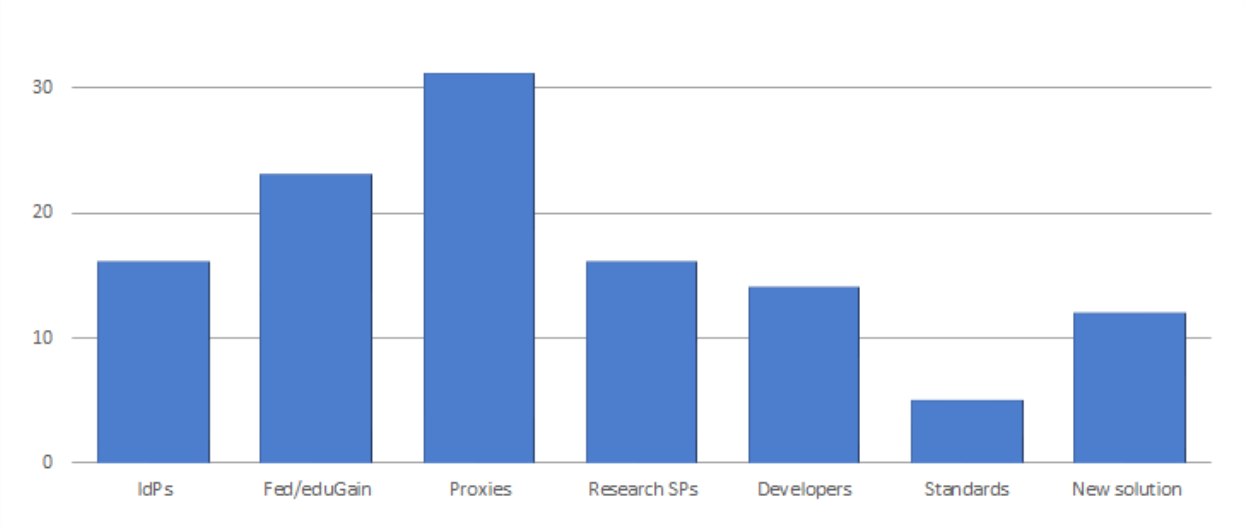
\includegraphics[width=0.7\columnwidth]{RequirementsBreakdown.png}
  \caption{Distribution of Requirements}
  \label{fig:breakdown}
\end{figure}

\subsubsection{Relative Importance of the Requirements}

Representatives of research communities present at the February 2018 FIM4R meeting were asked to indicate which of the requirements were of particular importance to them, i.e., not just ``all", as one indicator of breadth of impact that implementation of each requirement might be expected to have. Figure \ref{fig:voting} shows the number of different research communities so indicating, by each requirement. This ``vote" reflects a point in time for those research communities present at that meeting, representing less than half of those taking part in data gathered for this paper.

It is noteworthy that the top two reflect keen interest in research communities having direct representation in federation governance and in release of R\&S attributes by identity providers. One of the next two highest, Sirtfi adoption, likewise reflects how critical identity and federation operations are to research communities. The other, ORCID, reflects increasing uptake of ORCID both as an identifier that researchers are now expected to have and as an identity provider for researchers who may have insufficient, or absent, identity provider support by their home organisation.

Not all preferences counted necessarily reflect the degree of prospective impact. For example, Snctfi garnered only 1 ``vote"; however, the need for Research Community Proxies to be admitted to federation had a strong showing, and Snctfi is likely a key component of addressing that need. Some communities may have chosen to ``vote" only for the one knowing that it depends on the other, effectively getting two votes for one. As another example, although Help Desk, that is now operated by eduGAIN, received only 2 ``votes", that might mean it was generally taken for granted given that eduGAIN is already running a Help Desk. 

\begin{figure}[ht!]
  \centering
  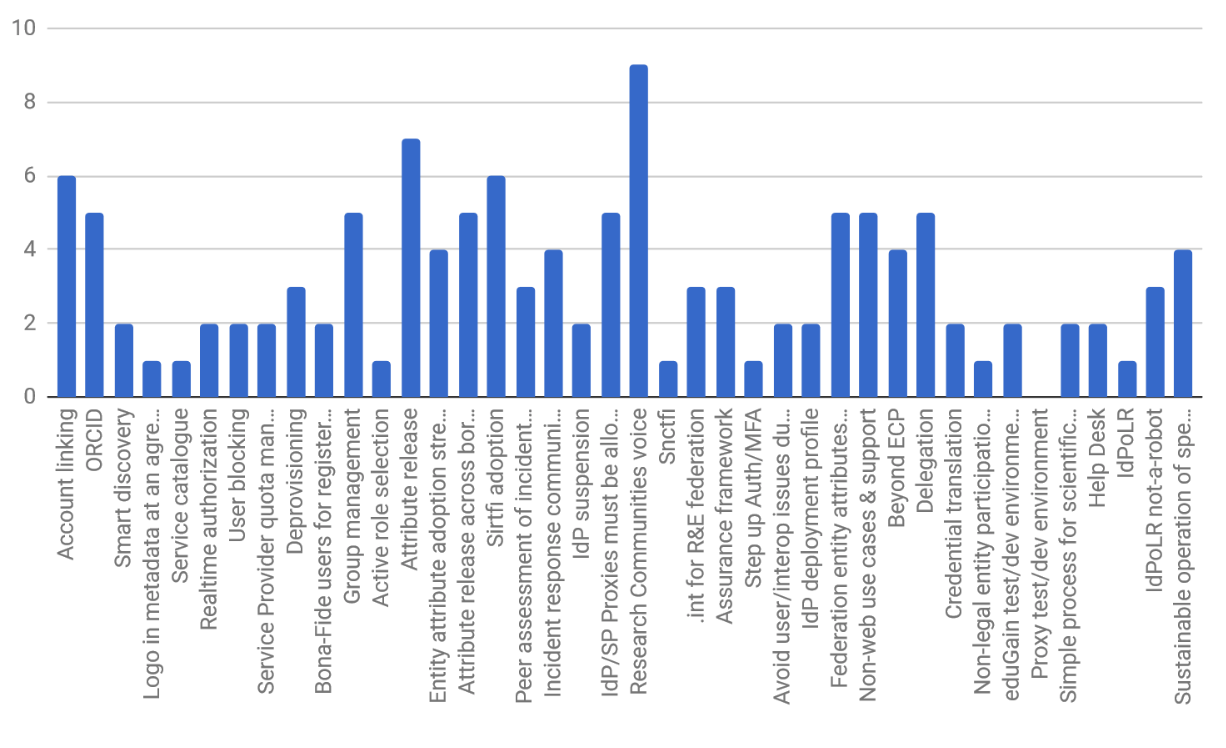
\includegraphics[width=0.7\columnwidth]{RequirementsVoting.png}
  \caption{Requirements Voting}
  \label{fig:voting}
\end{figure}

\section{Recommendations}
A number of outcomes are necessary to achieve the common vision of federated identity management, based on the requirements gathered above. All depend upon the substantial participation and cooperation of several groups, reflective of the evolved and evolving layers of technologies and services that comprise FIM. Each recommendation is expected to have broad positive impact on the viability and value of FIM for support of research going forward. A summary of which groups are mentioned in connection with each recommendation is provided in the section Mapping of Groups to Recommendations at the end of this section.
\subsection{Governance and Coordination}
\subsubsection{Increase research representation in FIM governance}
Organisations that envision or sustain critical FIM operations should plan and prioritise with input from all key stakeholders, including funders, planners, operators, architects, engineers and representatives of those to whom value of FIM is intended to accrue. At the time of this writing, some of the larger organisations in this space, such as GÉANT, Internet2, and some national R\&E federations, include few researchers or research e-Infrastructure operators among those they consult with or are governed by. This has contributed to an increased focus on developing R\&E federation to support enterprise applications. While that is valuable, it is incidental to the research and scholarly aspects of the academic mission. The expense and effort to provide a trustworthy infrastructure on which to securely manage collaborative access to research assets should be substantially undertaken by organisations whose mission it is to provide operational support to help enable research. Having sufficient research representation in their governance and advisory functions helps ensure the continued alignment of their actions with that mission.
\subsubsection{Sustain operation of critical FIM services}
The availability of FIM is increasingly critical for researchers to perform their workflows. It is essential that FIM services be operated sustainably, reliably and with a level of user support appropriate for the breadth of research use cases. Testing environments, help desks and accessible documentation are highly important for new communities to navigate the policies and technologies underpinning FIM. 

The footprint of what needs to be sustained is also increasing as new elements of the overall FIM ecosystem become critical to research workflows. Researcher and research e-Infrastructure operator participation in an organisation’s governance processes can help identify operations that have become critical to the overall research enabling ecosystem and assess consonance with the organisation’s mission and its existing services to focus effort to create business or funding models to sustain them. 

By suitably highlighting and including FIM as direct costs for projects, programs, and solicitations, research funding bodies can also bring substantial influence and focus to critical FIM capabilities that should be sustained.
Future e-Infrastructure projects should develop an interoperable mesh of complementary AAI solutions, building upon recognised best practices and supporting global research needs. The diversity of the research communities should be reflected in the AAI offerings; we do not see a single solution as a sustainable future. 
\subsubsection{Provide avenues for ongoing coordination} 
To produce and maintain current and coherent actionable plans, collaboration among parties across the FIM ecosystem, including federations, research e-Infrastructures, and research communities, should be on a continuing rather than episodic basis. Interested parties who sustain FIM and AAI operations should programmatically establish avenues for this ongoing coordination.

The mutual benefit of exchanging AAI experiences has been felt both by the research communities themselves and by the wider community, as projects and initiatives have been generated to resolve common issues. Such a forum should continue to be owned, supported and attended by research communities.  

\subsection{Baseline of Research User Experience}
Every researcher is entitled to focus on their work and not be impeded by needless obstacles nor required to understand anything about the FIM infrastructure enabling their access to research services. The recommendations in this section highlight well-established practices by home organisations and R\&E federation operators whose widespread adoption would represent a huge boost to usability of federated access mechanisms by users engaged in collaborative research activities. 

\subsubsection{Release Research \& Scholarship attributes}
Some research communities rely on their underlying proxies to obtain basic user attributes directly from users when users’ home organisations do not supply them. However, the value of federation is maximised when all home organisations participate in the R\&S Entity Category , removing that impediment from downstream operations and from the users. R\&E federations should increase efforts to get all of their identity provider members who employ researchers and scholars to participate in this well-established program.

To help identity providers in the EU address their obligations under the GDPR and so remove a further obstacle to releasing R\&S attributes, research service providers and proxies that directly participate in any R\&E federation and whose users include EU citizens and residents should support the Data Privacy Code of Conduct by implementing its recommendations and asserting a corresponding entity tag in their federation metadata. R\&E federation operators must offer their service provider members a satisfactory means of adding this tag to their entity metadata.

\subsubsection{Provide usability essentials}
Identity and service provider logos help users find their way and error URLs help them to get the right person’s attention when something goes wrong. R\&E federation members should ensure that all of their entity metadata includes these basic aides to good user experience. R\&E federation operators can help by making this the objective of outreach campaigns with their members.

\subsubsection{Remove interoperability barriers in eduGAIN metadata processes}
Users from different home organisations are not always able to access the same set of services because of the diversity of inconsistent practices followed by R\&E federations in their handling of eduGAIN metadata. eduGAIN receives entities exported by each R\&E federation and publishes an aggregate  metadata  file  that R\&E federations each import and publish within their federations.  Different R\&E federations implement different policies for determining which of their entities to export to eduGAIN, and similarly some R\&E federations filter some entities from the eduGAIN aggregate before publishing the result to their members. When a research service is not exported to eduGAIN, no users from other R\&E federations can access that service. When a research service is filtered, no user in the local federation can access it. When an identity provider is filtered, its users cannot access research services within the local federation.

R\&E federation operators should harmonise their eduGAIN export/import practices and ensure that eduGAIN itself addresses risks presented by entities sourced elsewhere, rather than each R\&E federation doing so unilaterally. All R\&E federations should support the ability of researchers and scholars at their member identity providers to access research services they need for their work.

\subsubsection{Admit research organisations to federation}
Some research e-Infrastructure operators and research communities that are not legal entities also do not have their FIM interests represented by a legal entity participating in an R\&E federation that can act on their behalf. This lack of legal standing can result in not meeting membership requirements for their national R\&E federation, which precludes associated research communities from benefiting from FIM. Similarly, some research organisations, legally recognised or not, are intrinsically and essentially transnational, not aligned with membership of any specific national R\&E federation. One or more R\&E federations, or perhaps eduGAIN, should provide reasonable processes to include such cases into FIM and widely promulgate them across R\&E federation operators. That way a positive answer can be given to the initial overture from such an organisation seeking to benefit from FIM.

\subsubsection{Enable researcher mobility}
Researchers change home organisations more often than they change their research domains or collaborations with colleagues. Research community proxies should support account linking techniques that enable a researcher to continue their appropriate access to research resources across such transitions. ORCID IDs should also be leveraged for this purpose.

\subsection{Security Incident Response Readiness}
Organisations participating in R\&E federations should apply best practices in operational security to their federated entities. They should also participate in security incident response frameworks such as Sirtfi and should be supported by their R\&E federation operators in doing so.

Each R\&E federation operator, and the eduGAIN operator, should have a security incident response plan. These plans should be tested periodically.

\subsection{Harmonisation of Research Community Proxy Operations and Practices}
Research community proxies emerged partly in response to needs unmet by R\&E federation and eduGAIN. This part of the FIM ecosystem is now maturing and has become a critical part of the FIM ecosystem; hence stability, support, and sustainability are now at least as important as continued innovation. These objectives are facilitated by avoiding the development, maintenance, and support costs associated with unnecessary duplication and non-essential differences.

\subsubsection{Follow the proxy model and related AARC guidelines}
The AARC BPA reflects the many successful proxy innovations produced by the research e-Infrastructure community. Continued innovation, such as further development of federated solutions for non-web use cases, should build on this model. Guidelines covering a variety of operational practices were produced and should be followed by proxy operators.

\subsubsection{Re-use shared AAI and related services} 
The technical skills for AAI development are scarce and the effort and time required for developing new AAI implementations is often underestimated. Research communities and research e-Infrastructure operators are strongly encouraged to use shared AAI services and related components, such as token translation and group management. Some research e-Infrastructures make AAI services generally available to research communities; these should be assessed for adoption before deciding to create any further instances that essentially duplicate what is already available. All large-scale e-Infrastructures are encouraged to make AAI services generally available to research communities. That said, we recognise that there will continue to be a need for some diversity of research e-Infrastructures, including research community proxies within them, to meet the needs of research communities subject to funding, geographical, or other substantive constraints.

Research communities within aligned domains are strongly encouraged to facilitate this re-use by collaborating to govern and sustain operation of a minimal set of enabling proxies and e-Infrastructures sufficient to support their research activities. 

\subsection{Sensitive Research User Experience}
The research community has substantial need to employ strong forms of authentication and access control to manage confidentiality of restricted research data sets and of preliminary results prior to publication, integrity of basic scientific data to ensure fidelity of its influence on public policy and to preserve academic attribution, and availability of specialised and expensive instruments and computing resources. Identity provider organisations are encouraged to provide strong authentication credentials to their researchers and implement the REFEDS MFA Profile to enable research service providers and proxies to signal when a user needs strong authentication to continue their activity and to acknowledge whether that has occurred. Identity assurance frameworks such as the REFEDS Assurance Framework should continue to be developed to respond to these needs.

\subsection{Mapping of Groups to Recommendations}

\begin{center}
\begin{longtable}{|p{0.3\textwidth}|p{0.7\textwidth}|} 
\hline
Groups & Recommendations \\ \hline \hline
GÉANT, Internet2, NRENS &  
Increase research representation in FIM governance \newline
Sustain operation of critical FIM services\newline
Provide avenues for ongoing coordination \\ \hline

Research funding bodies & 
Sustain operation of critical FIM services\newline
Provide avenues for ongoing coordination \\ \hline

Home organisations & 
Release Research \& Scholarship attributes\newline
Provide usability essentials\newline
Security Incident Response Readiness\newline
Sensitive Research User Experience \\ \hline

R\&E federations & 
Increase research representation in FIM governance\newline
Sustain operation of critical FIM services\newline
Provide avenues for ongoing coordination\newline
Release Research \& Scholarship attributes\newline
Provide usability essentials\newline
Remove interoperability barriers in eduGAIN metadata processes\newline
Admit research organisations to federation\newline
Security Incident Response Readiness \\ \hline

eduGAIN operator & 
Remove interoperability barriers in eduGAIN metadata processes\newline
Security Incident Response Readiness\\ \hline

Research e-Infrastructures& 
Sustain operation of critical FIM services\newline
Re-use shared AAI and related services \\ \hline

Research community proxies & 
Enable researcher mobility\newline
Security Incident Response Readiness\newline
Follow the proxy model and related AARC guidelines\newline
Re-use shared AAI and related services\newline
Sensitive Research User Experience \\ \hline 

Research communities & 
Re-use shared AAI and related services\\ \hline

REFEDS & 
Sensitive Research User Experience \\ \hline

\caption{Requirements Mapping}
\label{tab:mapping}
\end{longtable}
\end{center}

\section{Next Steps}
We plan to publish a version 2.1 of this paper, which will address any comments, additions and amendments communicated to the editing board by new communities that have not yet taken part in this FIM4R activity. To contact the editorial board, please use the contact details that can be found at fim4r.org. Although this version 2 already encompasses more communities than version 1, we feel that the group is still far from complete. We herewith call all research infrastructures that do see or at least begin to see the necessity of FIM for opening their user base but still want to have control on access to resources to add their own new requirements or to emphasise the requirements listed in this version. Although domain specific research e-Infrastructures are the main focus of this activity, other groups working on cross-domain infrastructures and technologies (The Research Data Alliance, RDA, for example) are also herewith encouraged to provide input to the next version of this text. 


\begin{flushleft}
\bibliography{fim4r}
\end{flushleft}

\section{Acknowledgements}
The authors acknowledge the contributions to this work made by all former members of the FIM4R collaboration. In particular, we thank Bob Jones from CERN, for his vision and leadership during the FIM4R v1 era, and for his contributions to Version 2. We also wish to thank colleagues, too many to name individually, in REFEDS, in GN4, among the national federations, the providers of identity management software, and the operators of many diverse Trust and Identity services for their endeavours to meet our FIM4R requirements. Additional thanks to Heather Flanagan of Spherical Cow Consulting for her time spent proof reading.

The authors also acknowledge the support and collaboration of many other colleagues in their respective institutes, research communities and IT Infrastructures, together with the funding received by these from many different sources. These include but are not limited to the following: (i) The Worldwide LHC Computing Grid (WLCG) project is a global collaboration of more than 170 computing centres in 43 countries, linking up national and international grid infrastructures. Funding is acknowledged from many national funding bodies and we acknowledge the support of several operational infrastructures including EGI, OSG and NDGF/NeIC. (ii) EGI acknowledges the funding and support received from the European Commission and the many National Grid Initiatives and other members. EOSC-hub receives funding from the European Union’s Horizon 2020 research and innovation programme under grant agreement No 777536. (iii) The work leading to these results has received funding from the European Union’s Horizon 2020 research and innovation programme under Grant Agreement No. 730941 (AARC2). (iv) Work on the development of ESGF’s identity management system has been supported  by The UK Natural Environment Research Council and funding from the European Union's Seventh Framework Programme for research, technological development and demonstration through projects IS-ENES (grant agreement no 228203) and IS-ENES2 (grant agreement no 312979). (v) Ludek Matyska and Michal Prochazka acknowledge funding from the RI ELIXIR CZ project funded by MEYS Czech Republic No. LM2015047. (vi) Scott Koranda acknowledges support provided by the United States National Science Foundation under Grant No. PHY-1700765. (vii) GÉANT Association on behalf of the GN4 Phase 2 project (GN4-2). The research leading to these results has received funding from the European Union’s Horizon 2020 research and innovation programme under Grant Agreement No. 731122(GN4-2). (viii) ELIXIR acknowledges support from Research Infrastructure programme of Horizon 2020 grant No 676559 EXCELERATE. (ix) CORBEL life science cluster acknowledges support from Horizon 2020 research and innovation programme under grant agreement No 654248. (x) Mirjam van Daalen acknowledges that the research leading to this result  has been supported by the project CALIPSOplus under the Grant Agreement 730872 from the EU Framework Programme for Research and Innovation HORIZON 2020. (xi) EISCAT is an international association supported by research organisations in China (CRIRP), Finland (SA), Japan (NIPR), Norway (NFR), Sweden (VR), and the United Kingdom (NERC).


\appendix
\newpage

%fim4rv2-authors-appendix.tex

\section{Appendix: Authors}  \label{Authors}

Table \ref{tab:authors} lists the ORCID identifiers of the Authors and also lists affiliations to Research Communities, e-Infrastructures and others; see also table \ref{tab:Communities}.

\begin{center}

\newcolumntype{C}[1]{>{\centering\arraybackslash}p{#1}}
\begin{longtable}{|p{5cm}|C{6cm}|C{2cm}|C{2.5cm}|} 


\hline
Name
&ORCID{\textsuperscript{\textregistered}} ID
&Research Communities
&e-Infrastructures and others \\
\hline
\hline
\endhead
%C J Atherton
Christopher John Atherton
&https://orcid.org/0000-0001-8223-6292
&
&63\\
\hline
%T Barton
Thomas Barton
&https://orcid.org/0000-0003-1878-3448
&
&65\\
\hline
%J Basney
Jim Basney
&https://orcid.org/0000-0002-0139-0640
&
&\\
\hline
Daan Broeder
&https://orcid.org/0000-0002-8446-3410
&41
&\\
\hline
%A Costa
Alessandro Costa
&https://orcid.org/0000-0003-0344-8911
&42
&\\
\hline
%M van Daalen
Mirjam van Daalen
&https://orcid.org/0000-0002-9648-7508
&52
&61\\
\hline
%S O M Dyke
Stephanie Dyke
&https://orcid.org/0000-0001-5756-3822
&47
&\\
\hline
Willem Elbers
&https://orcid.org/0000-0002-0191-9102
&41
&\\
\hline
%C-F Enell
Carl-Fredrik Enell
&https://orcid.org/0000-0003-1006-2822
&46
&61 62\\
\hline
%E M V Fasanelli
Enrico Maria Vincenzo Fasanelli
&https://orcid.org/0000-0002-1741-8011
&
&\\
\hline
%J Fernandes
J Fernandes 
&https://orcid.org/
&
&64\\
\hline
%L Florio
Licia Florio
&https://orcid.org/0000-0002-0919-410X
&
&61 63\\
\hline
%P Gietz
Peter Gietz
&https://orcid.org/0000-0002-8310-2015
&43
&61\\
\hline
%D L Groep
David L. Groep
&https://orcid.org/0000-0003-1026-6606
&
&61 62\\
\hline
%M Junker
Matthias Bernhard Junker
&https://orcid.org/0000-0003-2609-2698
&50
&\\
\hline
%C Kanellopoulos
Christos Kanellopoulos
&https://orcid.org/0000-0002-8939-2607
&
&61 62 63\\
\hline
%D P Kelsey
David Kelsey
&https://orcid.org/0000-0001-6712-4321
&55
&61 62\\
\hline
%P J Kershaw
Philip Kershaw
&https://orcid.org/0000-0002-7646-291X
&45
&\\
\hline
%C Knapic
Cristina Knapic
&https://orcid.org/0000-0002-4752-6777
&53
&\\
\hline
%T Kollegger
Thorsten Kollegger
&https://orcid.org/0000-0003-2145-0951
&48
&\\
\hline
%S Koranda 
Scott Koranda
&https://orcid.org/0000-0003-4478-9026
&51
&\\
\hline
%M Linden
Mikael Linden
&https://orcid.org/0000-0002-3634-3756
&47
&61\\
\hline
%F Marinic
Filip Marinic
&https://orcid.org/0000-0001-9754-8846
&44
&\\
\hline
%L Matyska
Ludek Matyska
&https://orcid.org/0000-0001-6399-5453
&47
&62\\
\hline
%T H Nyrönen
Tommi Henrik Nyr\"{o}nen
&https://orcid.org/0000-0002-5569-5183
&47
&61\\
\hline
%S Paetow 
Stefan Paetow
&https://orcid.org/0000-0001-5901-5256
&52
&61\\
\hline
%L Paglione
Laura A D Paglione
&https://orcid.org/0000-0003-3188-6273
&
&66\\
\hline
%S Parlati
Sandra Parlati
&https://orcid.org/0000-0001-7099-0378
&50
&\\
\hline
%C Phillips
Christopher Phillips
&https://orcid.org/0000-0001-5567-4916
&
&\\
\hline
%M Prochazka
Michal Prochazka
&https://orcid.org/0000-0001-8376-9533
&47
&62 63\\
\hline
%N Rees
Nicholas Rees
&https://orcid.org/0000-0001-7822-8150
&53
&\\
\hline
%H Short
Hannah Short
&https://orcid.org/0000-0003-2187-0980
&55
&61\\
\hline
%U Stevanovic
Uros Stevanovic
&https://orcid.org/0000-0001-7255-3294
&
&61\\
\hline
%M Tartakovsky 
Michael Tartakovsky
&https://orcid.org/0000-0002-8132-9013
&49
&\\
\hline
%G Venekamp
Gerben Venekamp
&https://orcid.org/0000-0003-3335-3390
&
&61\\
\hline
%T Vitez
T Vitez
&https://orcid.org/
&
&\\
\hline
%R Wartel
Romain Wartel
&https://orcid.org/0000-0002-0878-5303
&55
&\\
\hline
%C Whalen
Christopher Whalen
&https://orcid.org/0000-0002-1379-7392
&49
&\\
\hline
%J White
John White
&https://orcid.org/0000-0001-5614-0895
&46
&\\
\hline
%C Zwolf
Carlo Maria Zw\"{o}lf
&https://orcid.org/0000-0002-5762-6747
&54
&\\
\hline
                                       
\hline
\caption{Author details}
\label{tab:authors}
\end{longtable}

%\end{center}

 % \end{tabular}
%\newline\newline61
%\caption{Authors}
%\label{tab:authors}
%\end{longtable}



\newpage
%\begin{center}
\begin{longtable}{|C{0.8cm}|p{12.0cm}|} 
\hline

&\textbf{Research Communities}\\
\hline
\hline
\endhead

41 & Common Language Resources and Technology Infrastructure (CLARIN)\\
\hline
42 & Cherenkov Telescope Array (CTA)\\
\hline
43 & Digital Research Infrastructure for the Arts and Humanities (DARIAH)\\
\hline
44 & Earth Observation (EOP/ESA)\\
\hline
45 & Earth System Grid Federation (ESGF) \& Climate Science\\
\hline
46 & European Incoherent Scatter Scientific Association (EISCAT) \& EISCAT\_3D\\
\hline
47 & ELIXIR - a distributed infrastructure for life-science information\\
\hline
48 & Facility for Antiproton and Ion Research (FAIR)\\
\hline
49 & Infectious Disease Research\\
\hline
50 & Laboratory for Underground Astrophysics (LUNA) Collaboration\\
\hline
51 & Laser Interferometer Gravitational-wave Observatory (LIGO) Scientific Collaboration\\
\hline
52 & Photon and Neutron Facilities\\
\hline
53 & Square Kilometre Array  (SKA)\\
\hline
54 & Virtual Atomic and Molecular Data Center (VAMDC)\\
\hline
55 & Worldwide Large Hadron Collider Computing Grid (WLCG)\\

\hline
\hline

%     &  {e-Infrastructures and others}
&\textbf{e-Infrastructures and others}\\
\hline
\hline
61 & AARC/AARC2\\
\hline
62 & EOSC-hub\\
\hline
63 & GÉANT\\
\hline
64 & HNSciCloud\\
\hline
65 & Internet2\\
\hline
66 & ORCID\\
\hline

\hline                                           
\caption{Research Communities, e-Infrastructures and others}
\label{tab:Communities}
\end{longtable}
\end{center}



\newpage
\section{Appendix: Descriptions of Contributing Research Communities}

\subsection{Arts and Humanities}
The DARIAH (Digital Research Infrastructure for the Arts and Humanities)\cite{dariah} project is an ESFRI activity to design, set up and operate productively an infrastructure to support virtual research environments in the humanities, and thus furthers the digital humanities, a field that is being established to add new methods to all fields of humanities. DARIAH-DE, the German part of this all-European effort, runs an own IdP, as many users of the DARIAH infrastructure are ``homeless", i.e. they are not members of an organisation in a national federation or eduGAIN, or their organisation although being part of the federation, even refuses to release a permanent identifier to DARIAH services, which require the release of at least eduPersonPrincipalName. In any case, whether authenticated by her organisation or by the DARIAH IdP, the user will be redirected to a registration page when first attempting to use DARIAH services, so that the infrastructure retrieves needed attributes, such as email address, but also so that the user can consent to the DARIAH terms of use. The LDAP server that stores this additional information is also used to manage authorisation attributes such as privilege group memberships, that are consumed by DARIAH services for making access control decisions The DARIAH IdP can thus release all these attributes to the service via direct SAML Attribute Queries.

DARIAH provides a self-service interface that manages the registration process, but also allows for requesting an account, for changing the password, for getting a new password, when the user has forgotten the old one, for consenting to the DARIAH ToU, for registering additional attributes such as ORCID ID, and for applying privilege group memberships, mostly to get special access to special services, including consenting to respective special ToUs. An administration interface eases the distributed management of the data and the granting of the account and group management requests, respecting fine-grained role based access control.

The DARIAH guest IdP, which is included into the DFN AAI and thus also into eduGAIN, is operated according to a documented and publicly available policy for vetting the identities relating to participation in the research community and for keeping the data current. DARIAH also has a sustainability strategy for all services, including the operation of the IdP and its user management. 

In the first 5 years of production, all DARIAH SPs have operated in a mesh federation (DFN-AAI and eduGAIN) and deployment documentation exists on how to connect an SP to the DARIAH IdP using Attribute Queries. This put quite a burden to the DARIAH service developers and thus the uptake in many DARIAH-EU member countries was considerably slow. However, after the findings from the first phase of AARC culminating into the AARC Blueprint Architecture, DARIAH is currently (as of Q4-2017) shifting to a Proxy model based on an Shibboleth IdP-SP-Proxy developed by DARIAH-DE. This new proxy  allows for an easier integration of SPs and to more easily cope with federated IdPs not releasing eduPersonPrincipalName but only opaque persistent IDs targeted to a single SP (eduPersonTargetedID), because as to the IdP the proxy is the only visible SP and all actual SPs get the same targetedID. The proxy also allows for many more features, such as interoperating with different e-Infrastructures, like EGI, EUDAT and in future EOSC. A current pilot activity within phase two of AARC demonstrates such interoperability between DARIAH and EGI. Lastly the proxy will also help in future developments, such as providing the possibility of account linking, so that a user while switching her institution nevertheless can keep her rights within different DARIAH activities. 

In this way the work of AARC was very helpful for continuing the DARIAH AAI\cite{dariahaai} strategy already described in the first version of this paper, which on one hand secured interoperability with eduGAIN, but on the other hand allowed for productive operation by circumventing shortcomings of eduGAIN already at a very early stage. 

\subsection{Climate Science}
In this section on climate science we provide an update on developments with the Earth System Grid Federation (ESGF)\cite{esgf} first reported on in the original FIM4R paper. ESGF is a federated software infrastructure developed, deployed and operated by a number of participating organisations around the world for the purpose of disseminating model data and observations relating to the Earth system. At the time of writing for the first FIM4R report, data for CMIP5, the Coupled Model Intercomparison Project, phase 5 had been published into ESGF. CMIPs are organised under the World Climate Research Programme (WCRP) Working Group on Coupled Modelling (WGCM) have been run at regular intervals since 1995. The next phase, CMIP6 is underway. In each CMIP, modelling centres from around the world participate producing super-computer simulations conforming to an agreed common set of experiments. This enables scientists to share and compare models in order to better understand the earth system and predict future climate. The outputs and analyses are key to international assessments and negotiations for example providing input into IPCC assessment reports.

CMIP5 was the original driver for a federated infrastructure, recognising the challenges of providing access to such a large set of data (2.5PB) and ensuring it can be distributed as widely as possible to the science community for analysis. CMIP6 is no lesser challenge with projections of upwards of 40PB data output as a consequence of the use of higher resolution models and the incorporation of new processes.

Alongside this federated capability, for CMIP5 there was also the requirement for access control, to ensure users agree to terms of use for the data, to provide metrics to stakeholders and sponsoring organisations and in order to keep in contact with the user community to inform them of changes to the data. At the time, there was no federated infrastructure for identity management that could fully bridge international boundaries and meet the requirements for the programme. Consequently, participating organisations in ESGF developed and deployed a system based on standards and tools available at the time including OpenID 2.0, PKI for single sign-on and SAML 2.0.

The single biggest challenge for CMIP5 data access has been the ability to support non-browser based use cases and bulk data download. To meet the need to support both GridFTP and HTTP-based download a solution was developed based on SSL client authentication and short-lived user X.509 certificates. This enabled powerful scripts to be provisioned for users, to search for and download data distributed across the federation. However, it also proved problematic and complex for many users. Ultimately, users wanted friction-free access whilst at the same time, the need for per user download metrics on the part of data providers has been hard to justify against the development and operational effort to deploy and maintain a federated AAI.

Even so, in the intervening time since CMIP5, ESGF has been very successful, supporting a range of projects in the Earth Sciences domain. These include regional climate models and observations from satellite-borne instruments. Projects like the European Space Agency Climate Change Initiative Open Data Portal are built on the ESGF infrastructure but took the decision to have an open access policy for data. Looking forward, for CMIP6, all data will be publicly accessible without restriction. Licence terms will be embedded in the data and by downloading data, users agree to the terms of use contained.

Whilst the need for access control on many datasets is diminishing, the volumes of data being generated is providing a separate but related impetus for AAI. Observing the use of CMIP5 data since it was first published, there has been a trend away from individual user download towards aggregating data around regional computing facilities. The data is so large that users require dedicated facilities with sufficient computing resources alongside the data to enable them to perform their analyses. Within the ESGF technical roadmap, this had led to the development of a Compute Node, a software stack to enable users to execute processing at larger computing facilities remotely from their desktops. The focus then has shifted away from restricting access to data to restricting access to computing resources. This brings with it requirements for user delegation and the need for a greater level of assurance with user credentials and the authentication process.

Alongside ESGF, the need for hosted processing has been realised in the UK climate science and earth observation communities with the establishment of the CEMS (Climate and Environmental Monitoring from Space) and JASMIN facilities. JASMIN (http://jasmin.ac.uk) is a data intensive computing resource providing access to curated datasets like CMIP5 together with batch processing and a community cloud. Such a system enables direct access to data via a POSIX file system. Consequently there has been a need to rationalise access policy to allow for the limitations of POSIX access control semantics and unify this with existing access methods over HTTP and other protocols. Migration towards object storage and the use of public cloud for bursting scenarios present additional new challenges.

In the time since the first FIM4R report, technical advances, standardisation and increased support in the form of tooling and libraries have helped enormously. OAuth 2.0 is being used for ESGF and with JASMIN to support user delegation access scenarios. Both use an approach similar to CILogon, securing certificate issuing service with OAuth 2.0 thus providing a means to bridge to legacy services dependent on X.509-based user credentials. It is hoped to migrate towards OpenID Connect for SSO provision.

Systems for governance and operations have evolved and matured over the course of ESGF's development. It is moving to tiered approach with participating nodes committing to different service levels and service provision depending on the resources available to them. For the identity management system, the number of Identity Providers in the federation has been reduced recognising that only a smaller set of core institutions are able to commit to the long-term support of such services. Efforts around account linking between ESGF and institutional identities could provide further benefits reducing the operational overhead for the federation. The division of funding streams across national boundaries remains a challenge for the continuity of development but there are strengths in the established relationships in the community and shared goals.

\subsection{Earth Observation (EO)}

In the context of Space 4.0 and its ``EO Innovation Europe" concept, the European Space Agency (ESA), in coordination with other organisations, is forming a new ecosystem for exploitation of EO data under the name ``Network of EO Resources". The main goal is to bring the numerous and largely disparate EO datasets into a federated layer of exploitation platforms and enable the scientific users to perform research directly where the data is stored. Thus the current paradigm ``bring the data to the user" (users having to download enormous datasets to their premises and own massive infrastructures to process that data) will be replaced with the ``bring the user to the data" paradigm, as the exploitation platforms will not only provide the raw data, but also a computing framework with specific tools and algorithms relevant to Earth Sciences. An overview of the new ecosystem is shown in Figure \ref{fig:eo}.

\begin{figure}[ht!]
\centering
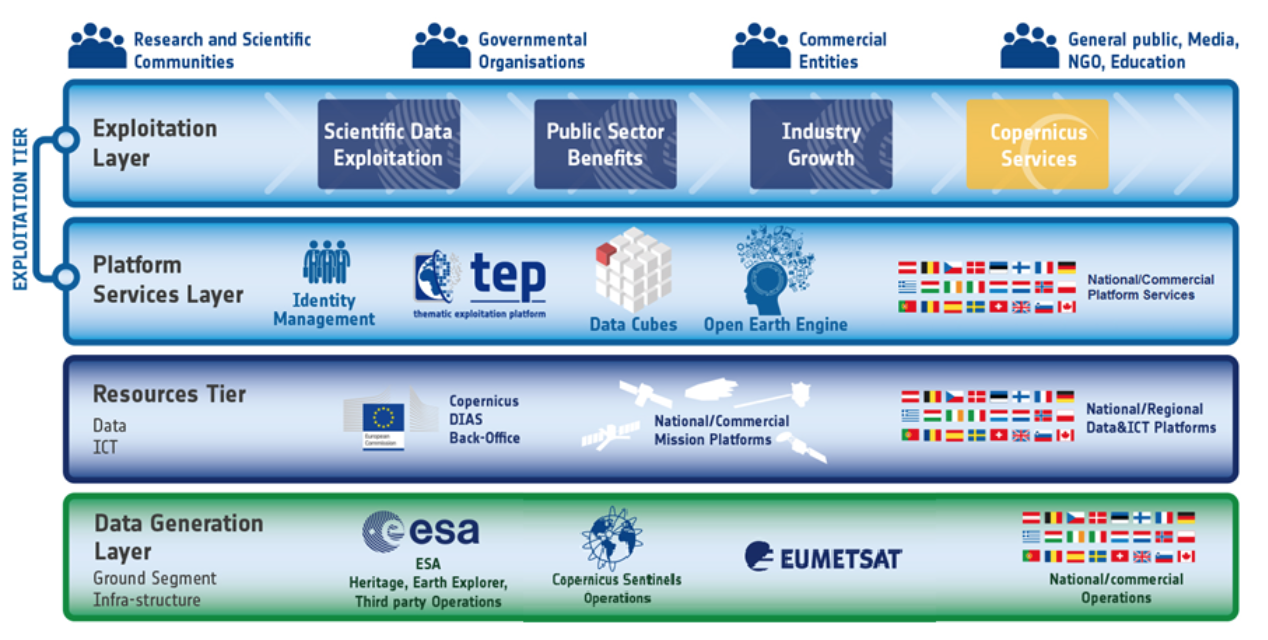
\includegraphics[width=0.7\columnwidth]{eo.png}
\caption{}
\label{fig:eo}
\end{figure}

Evidently, a Federated Authentication and Authorization Infrastructure is one of the key building blocks of this new ecosystem. In this context, ESA is currently running several Pathfinder activities with the aim to align the Federation approaches among the various players in the Earth Observation domain and ensure these approaches are in-line with the AARC Blueprint Architecture and the technical practices in eduGAIN.

For the operational phase, ESA plans to establish a Commercial Operator Identity Hub which shall provide federated identities to all EO users whose home organisations are not able to federate in any way. The Service Providers, members of the Network of EO Resources, shall federate directly with the Commercial Operator Identity Hub. In addition, a federation with eduGAIN and other inter-federations is encouraged.

Apart from the Earth Observation domain, ESA as an intergovernmental organisation has found it very difficult to join eduGAIN as a single entity, since no NREN can act as a central channel for all ESA sites located in various european countries. Currently the only option is to join eduGAIN via seven different national NRENs, each covering a subset of ESA Programmes. Such partitioning would be very counterproductive and confusing to the users not knowing which SP to select for which subset of the same Programme data. A solution to this problem is urged not only by ESA, but also by other similar organisations.

\subsection{European Neutron and Photon Facilities (umbrellaID)}
The umbrellaID system is a single-sign-on system managed collaboratively by 16 photon and neutron sources around Europe. Its purpose is to allow the large community of scientists using multiple facilities (i.e. >30000 users) for their experiments to share a single user ID across these facilities, irrespective of the actual usernames and passwords specific to the facilities. The amount of users of the umbrella ID is steadily growing at around 20\% per year. 
EC project initiatives such as CALIPSOplus and the new collaboration League of Accelerator based Photon Sources LEAPS, as well as upcoming projects within Horizon 2020 connected to the European Open Science Cloud EOSC intend to upgrade Umbrella ID to be a critical service for the facilities, and expand attribute usage, notably ORCID, which is quickly becoming a method tying paper submissions and publications to their source experiments and proposals, to the facilities, while the INSTRUCT ERIC and its BioStruct-X predecessor used the Umbrella ID as a light-weight alternative means to tie proposals submitted through it to the facilities and to ease the requirement to use multiple methods of logging into different facilities. Therefore Umbrella participates  in eduGAIN and projects such as GÉANT’s eduTEAMS and the EC-funded AARC and AARC2.
 
The system is very light-weight; at the moment it only releases three attributes to facilities in order to comply with the complex data protection requirements that are in place across Europe. Each facility continues to be the data controller and processor of the data held at the facility; the Umbrella ID merely enables single sign-on in the most simple sense of the word.
 
The umbrellaID system allows everyone to create an account on it but does not per se authorise a user to any service. The umbrellaID accounts can be linked with an existing account at a participating research facility and the umbrellaID account receives the authorisation the local account at the facility has. This also allows that an existing authentication and authorisation infrastructure still can be used.
 
The typical research team consists of a small number of researchers which gather data that belong solely to that small team and are not shared among other researchers until there is a publication. Some of the research can also be of commercial nature and therefore will never be shared. These specifics require special care in protecting the research data.
 
A crucial part in this system is non-web-based access. This need arises from the scientific workflow in this research field: proposal submission (web-based), data acquisition (non-web-based), data reduction and analysis (web-based), publication (web-based). The non-web-based access is realised with the Moonshot technology.

There is also a use case for umbrellaID to be used by other scientific communities, and this is a standing wish of the collaboration.

\subsection{Gamma-Ray Astronomy}
The Cherenkov Telescope Array (CTA) project aims to build a new generation ground-based observatory to cover the very high energy range of the universe.

The CTA concept was first proposed to the ESFRI (European Strategy Forum on Research Infrastructures) committee in 2006 as research infrastructure for gamma-ray astronomy with an estimated investment cost of around 150 M Euros (at 2006 cost levels). The CTA Consortium formed to design the instrument and to work towards its implementation. Since then the interest and the support for the project have grown, and currently the CTA Consortium consists of more than 1000 scientists and engineers in more than 160 institutions from 27 countries around the globe. CTA will answer many of the persisting questions by enabling the detection of more than 1000 sources over the whole sky. CTA builds on the proven technique of detecting gamma\-ray induced particle cascades in the atmosphere through their Cherenkov radiation, simultaneously imaging each cascade stereoscopically with multiple telescopes, and reconstructing the properties of the primary gamma ray from those images.\cite{cta-intro}
 
The participation of scientists from within CTA Consortium and from the greater worldwide scientific community necessitates a sophisticated scientific analysis system capable of providing unified and efficient user access to data, software and computing resources\cite{cta-data-man}.
The distributed scientific analysis system, including software and computing, require authentication and authorisation services to ensure security and privacy of data and resources.

\subsubsection{Implementation of the CTA AAI}
User requirements for the INAF-CTA AAI have been elicited first identifying the main Use Cases grouped in pre-defined criteria/categories such as ``Authentication capabilities", ``Account Management Capabilities", or ``Authorization capabilities" (see Figure \ref{fig:ctatable}. Thanks to the use cases definition, user needs have been identified towards the definition of user requirements.
 
\begin{figure}[ht!]
  \centering
  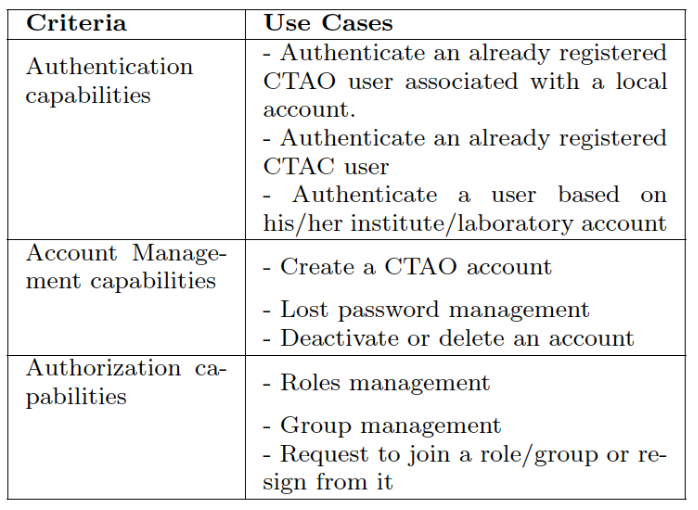
\includegraphics[width=0.7\columnwidth]{cta-table.png}
  \caption{Use case samples grouped by criteria}
  \label{fig:ctatable}
\end{figure}

The INAF-CTA AAI provides functionalities enforcing the protection of CTA resources and digital assets by means of a role based authorisation allowing both a federated  authentication, based on eduGAIN inter-federation, or a centralised CTA SAML authentication service. An attribute authority is also provided in order to allow a role based  authorisation based on a set of attributes managed and agreed at consortium level. This AA infrastructure offers a proper environment  for enforcing accountability  allowing  maintenance and audit of logs for relevant events.

The current implementation\cite{costa-jgc}  (see Figure \ref{fig:ctaaai} of the CTA Authentication and Authorization Infrastructure provisions more than 1000  consortium SAML identities and is releasing a persistent and non-reassignable ID as requested by CTA user requirements. 

\begin{figure}[ht!]
  \centering
  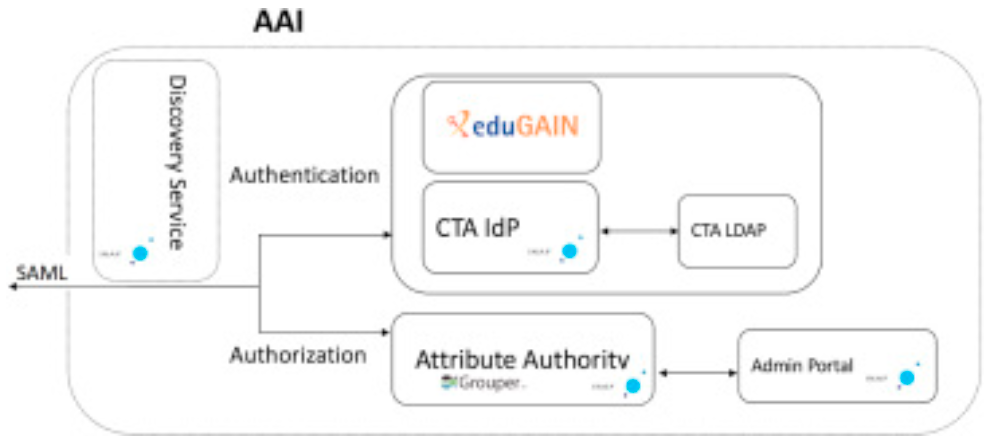
\includegraphics[width=0.7\columnwidth]{cta-aai.png}
  \caption{INAF-CTA AAI Architecture}
  \label{fig:ctaaai}
\end{figure}

The INAF-CTA discovery service facilitates the authentication by multiple IdPs. This is currently done by using the Shibboleth discovery service. The discovery service allows a service provider to identify the appropriate Identity Provider. The discovery service, starting from the federation metadata, provides the user with a list Identity Providers. A ``Search-as-you-type" selection offers an effective search that guides the user in creating and reformulating his/her selection.

On top of the eduGAIN federated authentication infrastructure INAF is providing a CTA Attribute Authority (AA) leveraging on Grouper\cite{COSTA2018}. This solution keeps information on user roles consistent across multiple applications. The IdP authenticates the user and issues a SAML assertion with a set of attributes. The authorisation is  is managed in a centralised way and is performed through a dedicated Attribute Authority which grants the definition, management and provisioning of roles based on groups and subgroups.

The infrastructure provides also web interfaces for group administration and web services allowing access to those functionalities in a service oriented architecture. 

\subsection{Gravitational Wave Astronomy}

\subsubsection{gw-astronomy.org}
The gravitational wave astronomy community has been preparing since 2007 for a global collaborative effort built on a foundation of federated identity. The LIGO Scientific Collaboration (LSC) group at the University of Wisconsin-Milwaukee (UWM) deployed a suite of tools, together colloquially known as ``gw-astronomy.org", that includes a federated identity collaboration registry, wiki, and email list server. The primary aim of the gw-astronomy.org platform is to facilitate collaboration between gravitational wave astronomers and astronomers from other fields including radio, gamma-ray, X-ray, and neutrino astronomy, in order to realise the promise of multi-messenger astronomy (MMA). The gw-astronomy.org platform not only facilitates collaboration through email lists and shared wiki access but also by managing authorised access to the LIGO Gravitational Wave Candidate Event Database (GraceDB). The gw-astronomy.org collaboration model based on global federated identity was validated by the collaborative work across the community resulting in the first MMA event that included observation of gravitational waves from a binary neutron star inspiral with electromagnetic counterpart on August 17, 2017.

The gw-astronomy.org service SPs are registered by UWM in the InCommon Federation metadata and injected into the eduGAIN metadata aggregate. Each SP is tagged in the metadata with the R\&S Entity Category to facilitate attribute release by eduGAIN IdPs. Collaborators may authenticate using any eduGAIN IdP that releases a persistent, non-targeted identifier to each of the SPs. Researchers without access to a federated IdP or an IdP that will release a persistent, non-targeted identifier may authenticate using a Google identity via a commercially managed social-to-SAML gateway service. Additionally the UWM LSC group has operated the LIGO Guest IdP for those researchers unable or unwilling to use a Google identity for authentication. The UWM LSC group had intended to decommission the LIGO Guest IdP in 2017 but has been unable to do so because of the need to provide federated identities to researchers working in countries that prohibit the use of Google services and that do not otherwise have access to a federated identity.

The primary issue facing the gw-astronomy.org suite of services is the number of eduGAIN IdPs that will not release a persistent, non-targeted identifier to the multiple services. As such the UWM LSC group plans in 2018 to begin transitioning the gw-astronomy.org services to using a proxy deployment architecture so that only the single proxy SP need be federated and can consume a persistent but targeted identifier for users.


\subsubsection{Laser Interferometer Gravitational Wave Observatory (LIGO)}
Since 2008 LIGO has provisioned LIGO identities, colloquially known as albert.einstein@LIGO.ORG identities, for all LIGO Laboratory and LIGO Scientific Collaboration (LSC) members and allowed them to be used for authentication with the LIGO IdP. While LIGO has joined the InCommon Federation and the LIGO IdP is published in the InCommon and eduGAIN metadata, to date the primary use of the LIGO IdP is for accessing the more than 70 LIGO SPs, most of which are not federated in InCommon and eduGAIN, with GraceDB and the main LIGO wiki being the notable exceptions.

Because of the growing success of eduGAIN and the proven gw-astronomy.org federated identity collaboration model, LIGO has recently undertaken, with financial support from the United States National Science Foundation (NSF), a three-year project to transition to leveraging global federated identity for access to LIGO SPs and de-emphasizing the role of the LIGO IdP. It is planned that at the end of the project LIGO identities used with the LIGO IdP will only be provisioned for a small subset of researchers to facilitate specific workflows at the LIGO interferometer sites and all other members of the LIGO Laboratory the LIGO Scientific Collaboration (LSC) will use federated identities from existing eduGAIN IdPs to access LIGO resources. In addition to the growth of eduGAIN, three other key factors that make the LIGO transition to federated identity tractable are the support for proxy architectures, the growing maturity of tools for managing federated identity, and the formation and growing adoption of the Sirtfi framework for security incident response.


\subsubsection{Virgo Collaboration}
Due in part to the data sharing agreement between Virgo and LIGO and the close collaboration of the two communities, LIGO has for years provisioned LIGO identities for Virgo scientists needing access to LIGO SPs. As part of the LIGO project to transition to fully leveraging eduGAIN and federated identity, Virgo users needing access to LIGO resources will use a federated identity and will no longer be provisioned a LIGO identity. Precisely which federated identities Virgo scientists will leverage and whether or not a ``Virgo federated identity" will be provisioned and a Virgo IdP published into eduGAIN is to be determined.


\subsubsection{Kamioka Gravitational Wave Detector (KAGRA)}
Because of LIGO's early investments in federated identity, it was decided years after the LIGO decision to provision identities for Virgo scientists when KAGRA scientists needed access to some LIGO resources to not provision LIGO identities but instead rely on federated access for KAGRA scientists. To facilitate the federated access of KAGRA scientists to LIGO resources the University of Tokyo deployed and operated the KAGRA IdP. Discussions are currently underway to understand how and when the KAGRA IdP may be replaced with federated access using eduGAIN IdPs not only for access to LIGO federated resources but also to KAGRA resources.

\subsection{High Energy Physics}
CERN, the European Organization for Nuclear Research, leads the World-wide LHC Computing Grid Project (WLCG) that provides the globally distributed computing infrastructure necessary for over 13,000 physicists to analyse and process the particle collision data from the Large Hadron Collider (LHC). The High Energy Physics (HEP) community is already successfully using federated identity in the form of x509 certificates, issued by CAs of the Interoperable Global Trust Federation (IGTF). Although x509 certificates have provided a good solution to the HEP community’s needs for distributed identity management, it is widely recognised that they pose usability problems for researchers and introduce security concerns related to the management of the researcher’s private key.

Non-x509 identities have become increasingly interesting to the HEP community, notably in the forms of SAML federations and interfederation, and stand-alone identity providers such as ORCID. The definition and adoption of Trust Frameworks, including Sirtfi, has built confidence in the potential for such identities to demonstrate an acceptable level of assurance. Several WLCG web services have already been integrated with CERN’s IdP-SP Proxy, and a working group has been established that will address non-web use cases.

Although progress has been significant, there is considerable effort required for WLCG to fully integrate non-x509 federated identities:
\begin{itemize}
\item Adoption of frameworks, such as Sirtfi, R\&S and ongoing work on assurance classification, by HEP participants is crucial for our researchers to possess a viable identity. 
\item Mature, tested procedures and tools for federated security incident response is needed. All parties involved - including organisations, federation and inter-federation operators - must provide security contact information and will be required to act through pre-established communication channels.
\item As dependence on the identity federation infrastructure itself grows, operational support is essential, including:
\begin{itemize}
\item A helpdesk that is well advertised and responsive.
\item Better guidance for service onboarding to identity federations and eduGAIN, for example services that provide Infrastructure as a Service (IaaS) for the research community.
\item An increased level of speed and flexibility to enable the adoption of community frameworks by identity federation participants. The inclusion of additional sources of authoritative information beyond federation registries is likely to support this requirement.
\end{itemize}
\item Critical, shared infrastructure components, including token translation services and VO Management, must be sustainably operated.
\item As infrastructure services move towards authorisation schemes, such as OAuth2 and JWT, federation support for standard tokens beyond SAML will aid interoperability. An Authorization Working Group has been established in WLCG to follow the impact of these changes.

\end{itemize}

\subsubsection{HNSciCloud}
The Helix Nebula Science Cloud Pre-Procurement Project\cite{hnscicloud} has developed a hybrid cloud platform that links together commercial cloud service providers and research organisations’ in-house IT resources via the GEANT network. The development work to address the R\&D challenges of the project has been performed by the cloud providers themselves in line with the requirements identified by the procurers, 10 research institutes invested in the concept of a hybrid cloud for the wider community. One of the main challenges was to setup access to the hybrid cloud compute services via SAML identity federation, specifically by enabling eduGAIN authentication, and becoming a relying party in the ELIXIR AAI. WLCG is one key use case for the hybrid cloud and the High Energy Physics Community has been represented through CERN as a procurer. 

During the design and prototype phase of the HNSciCloud Pre-Procurement project, several difficulties were encountered:
\begin{itemize}
\item There are multiple proxy implementations and service offerings to different communities with no clear understanding of the added value of each, or how sustainable the service offerings are. The commercial cloud services opt for developing/maintaining their own proxy service to ensure long-term sustainability.  
\item The lack of a real sustainable service makes eduGAIN on-boarding of Commercial Cloud Services very difficult. The problems are several: R\&S bundle use not clear, lack of central automated testing for SPs against IdPs, lack of central point of contact for operational support, lack of structured documentation for SP onboarding and overall service best practices.
\item Since ECP has largely been declared unsupported, there is no native command-line option. Research services wishing to use command line need to be connected to a complex AAI that follows the AARC blueprint, which is not suitable or feasible for some use cases. Alternatively, a native command line solution should be found.

Further experience with the deployment of FIM in a hybrid cloud model will be gathered by HNSciCloud during the pilot phase through to the end of 2018. 

\end{itemize}

\subsection{Ionospheric and Atmospheric Science}
The EISCAT Scientific Association (EISCAT) will establish EISCAT\_3D, a system of distributed phased array radars that will enable comprehensive three-dimensional vector observations of the atmosphere and ionosphere above Northern Fenno-Scandinavia. The use of new radar technology, combined with the latest advances within digital signal processing, will achieve ten times higher temporal and spatial resolution than obtained by the present EISCAT radar systems while simultaneously offering, for the first time, continuous measurement capabilities. The flexibility of the EISCAT\_3D system will allow the study of atmospheric phenomena at both large and small scales unobtainable by the present systems.

The EISCAT\_3D system will, in its first stage of construction, consist of three radar sites: one with both transmitting and receiving  capabilities and two with only receiving capabilities. The sites will be located in remote but easily accessible locations in three different countries (Finland, Norway and Sweden) and will be separated geographically by approximately 130 km. Two additional receive sites, at distances 200-250 km from the transmit site, are planned for the full EISCAT\_3D system at a later stage. 

In order to process and store the data acquired at the EISCAT\_3D radar sites, an operations centre, a control centre and two or more data centres are planned. The control centre is where the EISCAT\_3D scientists and engineers control and configure the radar transmitter and receivers. The EISCAT\_3D control centre will coordinate the radar operations and observation modes, monitor the production of the standard data products from the different sites, non-standard products, and the products that result from combining the measurements from the different sites (multi-static data products) from the operations centre. The control centre does not have to be a physical location but can be distributed, with authenticated operators accessing the system remotely.

The operations centre will be connected to the radar receive sites by fast (planned 100 Gb/s)
connections and consists of the 20 PB online disk buffer and up to  500 TFLOPS of computing by the year 2030. The operations centre computing is required for generation of non standard products as well as the products that result from combining the measurements from the di
erent radar sites (multi-static 3-dimensional data products). The operations centre will also generate any necessary additional metadata for the data les as well as the metadata catalogue(s), and transfers the data and metadata to the data centres for storage and curation.

The EISCAT\_3D data centres store the data products that are produced at the operations centre. This data is subsequently served to the EISCAT\_3D users for further analysis through the user portal. The data centres serve the data to users from either the fast data store (approx 5 years of data) or the slow data store that comprises the balance of the collected EISCAT\_3D data. At the data centres the data and metadata will be handled and catalogued by a data management system. The data centres will have to be tightly integrated with the user access portal and data (re)processing functions either at the operations centre or elsewhere.

\subsubsection{Current Implementation of EISCAT AAI}
EISCAT does not use a central AAI at this time. The current EISCAT radar systems have in the order of 100 users who actively analyze the data. Users access the processed data through the EISCAT Madrigal portal\cite{madrigal}. Archived lower level and raw data is accessed and downloaded through a Python/CGI web interface, which utilises a directory catalogue stored in a MySQL database. In the case of data that is under embargo, access control is implemented on IP address location. There is also a provision to computing access for analysis also under the same IP control, but local resources (desktop, laptop or institute clusters) are also suitable for analyzing EISCAT data. The portal also provides requests for radar operations. These are manually taken care of for actual scheduling of the radars.

\subsubsection{Future requirements for EISCAT\_3D AAI}
The AAI requirements for EISCAT\_3D are not particularly complex. The user base, space/atmospheric scientists performing the analyses, comes primarily from the EISCAT member countries and affiliate institutions, which are the Nordic countries (FI,NO,SE) as well as the UK, Japan, China, France, Ukraine and South Korea. EISCAT data are used world-wide, however, through collaboration with EISCAT scientists.

The scientific users are expected to access the data and computing capacity through a portal (currently the DIRAC interware is being prototyped and evaluated in the EOSC-hub project). The scheduling of EISCAT\_3D will need a more automated way of decisions, as the radar will run unattended and allow much shorter foresights of mode changes. These requests can come from human or machines interfaces. Actual operation of the radar transmitting and receiving sites will access the control system in a more direct fashion (ssh, command-line etc) but will also need to access higher level functionalities (graphic plots of real-time data collection) through portal-like interfaces.

It is most likely that the computing resources used for user analysis and even some of online data processing will be located in national e-Infrastructure provider (e.g. CSC in Finland) sites. 
Therefore it will be necessary to understand which users are using which resources (e.g. CPU, storage, network) as the EISCAT requires that usage records are generated and transferred to them for their accounting purposes. An AAI system is also necessary for the ``bookkeeping" of the data accesses of users and to prevent unauthorised usage of data. A traceable AAI login/identity will ease these necessary accounting tasks.

EISCAT does not anticipate the budget nor possess the expertise to manage credentials or virtual organisations. The EISCAT\_3D users must not be exposed to low-level credential handling (x.509 certificate/key or browser certificates etc). Therefore, the easiest mechanism for EISCAT\_3D users to authenticate and be authorised is to use their current  university/institutional login. Therefore the AAI for EISCAT\_3D must be minimally compatible with the national federations (SWAMID,Feide,Haka) of the participating countries and, considering the participation from outside the Nordics, eduGAIN.

The data that the EISCAT\_3D radars will produce will not be required to be stored in encrypted form but data transfers will be encrypted at the transport level. Some data will be embargoed anywhere from 1 to 3 years during which it is analyzed solely by the group that requested/paid for the experiment. After the embargo period, the data is released to the general EISCAT community for further analysis. Eventually, the data is to be released to the general public e.g. for citizen scientists. A further requirement on the AAI is that commercial AAI, such as a Google ID, should be able to access publicly-accessible data. A proxy for different authentication is being developed within the AARC2 project. 

\subsection{Infectious Disease Research}
\subsubsection{National Institute of Allergy and Infectious Diseases Virtual Research Organization Platform}
The National Institute of Allergy and Infectious Diseases (NIAID), one of the 27 institutes and centers that are the US National Institutes of Health (NIH), designed the Virtual Research Organization (VRO) platform as a way to support global research collaborations—in particular, their International Centers for Excellence in Research (ICERs)—that investigate emerging and re-emerging pathogens.  These and other centers supported by the NIAID form part of a global effort that crosses political and institutional boundaries to aid the struggle against infectious diseases and improve understanding the ecosystem of human immunity.  The NIAID built the three ICERs in collaboration with local research institutions in Bamako, Mali; Entebbe, Uganda; and Chennai, India.  These centers act as collaboration hubs for global research communities investigating the pathogens endemic in those regions.

The NIAID Office of Cyberinfrastructure and Computational Biology (OCICB) designed the virtual collaboration platform to solve some of the problems encountered over the 20 years that they have supported the ICER research programs and other global scientific efforts.  Infectious diseases do not respect political borders or geographic barriers.  An emerging pathogen in one remote part of the world can be in any city on any continent within 24 hours.  Few other scientific endeavors are as necessarily collaborative and international as this one. 

Collaborations depend on many resources that digital tools can either hinder or facilitate.  Common activities include developing funding proposals, protocol design, and sharing guidelines for research programs.  As data set sizes, types, and complexities increase, it becomes necessary to provide access to the toolsets and data to researchers around the world in a virtual laboratory.  Sponsors and publishers want to ensure that collected data sets are findable, accessible, interoperable, and reusable.  These FAIR principles are more easy for researchers to use if the common data models and standards integrate into the collaboration platforms like that developed by NIAID.

The ICERs provided the initial incentive to build the Virtual Research Organization platform.  They each have a high number of researchers from the NIAID intramural program who visit regularly and work with the local institution staff and scientists.  These collaborations often last years and include researchers at other academic institutions around the world.  Many of these investigators begin research in Mali, Uganda, or India while completing their training at the NIAID.  The U.S. research and education trust federation, InCommon, provided an identity and authentication framework that guided the development effort that allowed NIAID to use ICER and NIH identities to access research tools. InCommon also provides access to most of the U.S. academic institutions and, through eduGAIN, many of the international university faculty as well. 

Because NIAID administers the identity and access management infrastructure at the ICERs within the collaborating institutions, NIH sponsored them into InCommon metadata under the NIH membership.  However, many independent research institutions and foundations are unable to join their domestic trust federations as identity providers.  The uneven way that federations allow non-governmental organisations and non-academic institutions to be fully participating members of the federations continues to cause interoperability problems for the NIAID Virtual Research Organization Service Provider.

We also found that more than half of the identity providers in the global trust framework do not provide any attributes in the authentication assertion to the service provider.  Therefore, we were forced to create identities for many of the collaborators from those institutions.  These NIAID-created identities were also necessary for the scientific and clinical staff working at commercial or non-governmental organisations/research foundations.  Twenty percent of the institutions did provide an identity attribute for the collaborator in addition to the authentication.  Those identities can easily move from one service to another using the same authorisations that we set for groups of collaborators in the VRO.  However, we found that the remaining identity providers sent targeted identifiers that were unique for each service provider.  This data forced NIAID to install an identity provider/service provider proxy that would allow the use of a targeted identifier with all our service providers.  The proxy model also made it possible to use software and cloud services whose developers had only foreseen the need to support a single IdP in their SAML SSO integration.

Operating global collaborations includes collecting and characterizing data from multiple sites and locations, analyzing and storing that data, and moving the data and metadata from one research facility to another where tools and expertise exist.  Microsoft SharePoint, the first service provider supported by the NIAID VRO platform, addressed the primary need of a simple document management system.  This provided an easy way to deliver a service that allowed NIAID to map collaborations and laboratory staff from COmanage groups to SharePoint site collections and subsites.  Complicated protocols with multi-site collaborations can use multiple groups of different federated identities from around the world to control access to different levels of a SharePoint site.  For the African ICERs, NIAID installed a VRO SharePoint server at each location that allowed them to load data in at LAN speed.  Remote collaborators with more reliable, less congested internet connections can download during off-peak hours, made easier by time zone differentials.

At our Mali laboratories, we worked with the University of Science and Technology in Bamako to develop supporting infrastructure for the new graduate program in bioinformatics.  This required a high-performance server that supported distance learning, with the teachers for many of the courses delivering them remotely from various academic institutions worldwide.  The VRO infrastructure uses COmanage to store and distribute users' SSH public keys, which provide class participants and teachers access the bioinformatics environment configured for each of the courses according to the requirements of the instructor.  In the second African Center of Excellence in Bioinformatics, under construction in collaboration with Makerere University in Kampala, NIAID is building the platform with a cluster of servers using OpenStack and federated identity to access and use the guest instances.

One of the most important aspects of infectious disease research is collecting metadata from the field sites concerning the specimens, vectors, and hosts.  Traditional collection methods used paper forms that were manually transcribed into data management systems.  Even with the advent of electronic data collection from any internet-connected computer, ad hoc data models and ontologies make reuse of the data extremely difficult.  The current NIAID VRO uses REDCap, a remote data capture system built by Vanderbilt University with support from NIH grants, to support standard data models for research protocols that will make downstream use of the study data much easier, opening many possibilities for cross study analysis that were more difficult in the past.  In the future, this ``model-as-a-service" will continue the NIAID path to reduce the complexity of data management activities and increase use of standard models with other tools such as specimen management and data transfer.

The VRO platform has allowed the NIAID International research programs to begin the process of standardizing the scientific tools used at the ICERs in Mali, Uganda, and India as well as non-center based collaborations.  The identity providers at the three centers are now being used by services at the NIAID to allow access to collaboration and communication tools.  Engagement with national research and education network community in Africa and the other continents has also helped expand the understanding and use of federated identity by collaborators and academic institutions in these countries.


\subsection{Life Sciences}
A common Authentication and Authorisation Infrastructure (AAI) that would allow single sign-on to services across the BioMedical Science European Strategy Forum Research Infrastructure (BMS ESFRI) has been identified as a strategic target in the community.

\begin{center}
\begin{longtable}{|p{3cm}|p{5cm}|p{5cm}|}
\hline
\textbf{Infrastructure} &
\textbf{Domain of activity} &
\textbf{Website}\\ \hline \hline
\endhead
BBMRI&
Biobanking \& biomolecular resources &
www.bbmri-eric.eu\\ \hline
EATRIS&
Translational research&
www.eatris.eu\\ \hline
ECRIN&
Clinical trials&
www.ecrin.org\\ \hline
ELIXIR&
Curated databases&
www.elixir-europe.org\\ \hline
EMBRC&
Marine Biology and Ecology&
www.embrc.eu\\ \hline
EMPHASIS&
Plant phenotyping&
emphasis.plant-phenotyping.eu\\ \hline
ERINHA&
Highly pathogenic microorganisms&
www.erinha.eu\\ \hline
EuBI&
Biological/medical imaging&
www.eurobioimaging.eu\\ \hline
EU-OPENSCREEN&
Screening \& medical chemistry&
www.eu-openscreen.eu\\ \hline
INFRAFRONTIER&
Functional genomics&
www.infrafrontier.eu\\ \hline
INSTRUCT&
Structural biology&
www.structuralbiology.eu\\ \hline
ISBE&
Systems biology&
isbe.eu\\ \hline
MIRRI&
Microorganisms&
www.mirri.org \\ \hline
\caption{European Life Science Research Infrastructure stakeholders for AAI.}
\label{tab:lsstakeholders}
\end{longtable}
\end{center}

A concept of a Life Science AAI has been developed\cite{ls-ref} based on existing AAI implementations (e.g. ELIXIR AAI, BBMRI AAI and Instruct ARIA). The document describes the requirements of the Life Science AAI, and will be tested using the service portfolio for the research infrastructures participating in the biological and medical science ESFRI cluster (CORBEL, www.corbel-project.eu) and in the upcoming Life Sciences cluster in the European Open Science Cloud. 

The Life Science AAI requirements were developed with the CORBEL project and will be implemented in the AARC2 project. The Life Science AAI is based on the scientific use cases translated by the AAI experts of the participating research infrastructures. However, the Life Science AAI requirements are not particularly Life Science specific but could be easily translated to other disciplines who process sensitive data, such as humanities and social sciences. Work has received good feedback from the European e-Infrastructures such as GÉANT, EGI and EUDAT, who are preparing to respond to the service request.

\subsubsection{Reference Implementation AAI}
Scientists and other users can already use their existing user credential to create an ELIXIR ID\cite{elixir-aai}. ELIXIR AAI services allow users to link their federated academic, corporate or social media identity into a personal ELIXIR ID without creating a new username-password combination.  

This makes user and access management scalable for service providers who choose to trust the AAI services. Scientific service providers relying on ELIXIR AAI benefit from a centralised user identity and access management services. The growth rate for number of users and relying scientific services is rapid. Supported protocols are SAML2, OpenIDConnect.

\subsubsection{Sensitive data access models are evolving}
Reliable electronic authentication of users is a requirement to authorise access to the key services and instruments, sensitive data and computing capacities targeted to life science use. Technologies in access management are developing rapidly, and new concepts are needed globally to respond to requirements such as the EU GDPR without creating obstacles for research in e.g. human health.

The AAI infrastructure must thus support federated access to data that needs to be access-controlled. Access to sensitive data such as human data is typically mediated by an agreement between a data user and a data provider/controller. Access agreements take into account legal and ethical requirements, professional guidance, and good practices to enable use of data processors like secure cloud services. Agreements are in general executed by data stewards or data access committees, and could be implemented in electronic form employing software for identity and access management.\cite{Brandizi2017}\cite{Linden}
 
Some datasets like statistical averages are anonymous, and can thus be made public, with terms of usage if necessary. The middle ground between controlled access, whereby research plans and data access are approved on a case-by-case basis, and public access is however very wide. The genomics research community is developing a novel data access model, ``Registered Access", to bridge the realms of open access data and controlled data access review\cite{dyke}. Access to controlled datasets, such as those distributed by the European Genome-phenome Archive (currently maintained and deployed by EMBL-EBI and CRG), typically involves review and approval of researcher identity and research proposals for access to a single dataset for single use. This approach is not without difficulties. For example, it may be difficult to foresee all research goals at the time of the access decision and authorised use is often restricted by consent permissions. Further, at a time when genomic scientists aim to bring together multiple datasets from different studies to use for discovery or statistical inferences in a range of genome-wide analyses, these controls seem increasingly prohibitive as well as cumbersome. In Registered Access, researchers and other potential categories of data users (e.g., clinical care professionals) would be approved (registered) once, based on their identity and professional activity, for access to a range of data resources, as long as they followed standard community-wide data use conditions, such as keeping the data secure.

This data access model is being formalised and tested in the context of an international coalition of academic, public, and industry partners in genomics research, healthcare, and IT: the Global Alliance for Genomics and Health (GA4GH)\cite{ga4gh}. Its implementation - for bona fide researchers initially - will be piloted by GA4GH Driver Projects, notably ELIXIR Beacon, a network enabling the discovery of existing data on genetic variants, from both ELIXIR data resources as well as any Beacon-connected database anywhere. We see great opportunities to enhance genomics data access by expanding FIM systems to allow for several access control layers (e.g., bio/health researcher or ``registered" user) that would support Registered Access.

\subsection{Linguistics}
The CLARIN (Common Language Resources and Technology Infrastructure) ERIC is managing the CLARIN service provider federation (CLARIN SPF) and operating a homeless Identity Provider (CLARIN IdP). This was already reported on in the first FIM4R paper. Here we will provide an update on the improvements made to this infrastructure and on our experiences in operating it.

The CLARIN SPF has evolved tremendously since 2013, which current status is described in the CLARINPLUS Deliverable 2.7. The number of participating national identity federations (IDFs) has grown from a handful to 18 in mid 2017, enabling user's from 1577 organisations to use single sign-on to login to CLARIN services. The CLARIN SPF is intended to ease the administrative overhead for its service providers to connect to all the different national IDFs in countries with CLARIN users and should address  any issues for the federation as a whole. The two current main issues of the SPF, were already reported in the first FIM4R paper, are: (1) opt-in policies at the IDF level and (2) attribute release by the IdPs. 

CLARIN service providers publish their metadata to the SPF which then in turn is responsible for the provisioning of this metadata to all IDFs. Some IDFs have an opt-in policy which allows users of all the IDF’s IdPs access all connected SPs by default.  If an IDF does not have an opt-in policy or if the opt-in rate is high enough, typically above 50\%, the prefered way of publishing the SP metadata is via the German DFN federation into eduGAIN. The majority of IDFs, 12 out of 18, receive the CLARIN SPF metadata via this channel. For the remaining IDFs, 6 out of 18, the CLARIN SPF has joined the individual IDFs and is publishing metadata to each of them according to their specifications. For these federations the CLARIN SPF takes care to negotiate block opt-ins if possible, meaning that all CLARIN SPs are accepted as a single block when an IdP accepts a single one of the CLARIN SPs, but this is not always the case. While this reduces the administrative effort  for the individual service providers, this is not an easy task and puts an extra  burden on the CLARIN ERIC. Updates to the SPF metadata can be quite frequent and distribution to the national federations sometimes is a manual task with hard to use user interfaces.

As described in the CLARINPLUS Deliverable 2.7\cite{vanuyt}, common reasons for insufficient attribute release are related to privacy issues and a lack of trust from some of the Identity Providers. The set of required attributes itself, both required and recommended, by the CLARIN SPF has not changed since the publication of the  first FIM4R paper. As the operator of the SPF, CLARIN ERIC applies the following strategies to ensure the requested attributes are released to the CLARIN  service providers:
\begin{itemize}
\item Maximise SP acceptance by implementing trust enhancing policies
\item Ensure our service providers follow Data Protection Code of Conduct.
\item Through the Research and Scholarship entity category CLARIN indicates it uses the personal attributes solely for research purposes.
\end{itemize}

Thanks to work done in CLARIN-PLUS\cite{Mistuka} statistics are kept about which Identity Providers are not releasing attributes. These are contacted with a polite request to provide the attributes.

The main conclusions from CLARINPLUS Deliverable 2.7 on the attribute release issue are:
The attribute release issue is not as big as it is sometimes pictured (for the service providers in the CLARIN SPF, percentage of IdPs not releasing personal attributes: 10\% for UFAL, 18\% for HZSK, 0\% for Korp / CSC, 11\% for CLARIN.SI).

The problem varies widely among the national federations, with Germany being the most problematic case (7 out of 17 for UFAL, 6 out of 8 for HZSK, 1 out of 3 for CLARIN.SI)

Despite the increase of the number of IDFs accepting SPs from  the CLARIN SPF, there still are user's without the possibility to access services at a CLARIN SP.  Partly caused by users lacking an account at one of the institutions covered by the connected IDFs. Or because of the attribute release issue, where the user institute’s  IDP does not release the required attributes. Therefore the need for a ``homeless" IDP still exists today. CLARIN ERIC is operating this homeless IDP for the CLARIN SPF which  is run on a best-effort basis and accounts have to be verified on an individual basis. Although the technical effort required to operate this IDP is quite low, the administrative effort of verifying these user accounts and answering end-user support questions is much higher.

Although attempts have been made to leverage the CLARIN SPF also in providing access to web services using OAUTH2 but this has until now not resulted in a ready to use service. In the context of the EUDAT2020 project attempts were made to integrate the CLARIN SPF with the EUDAT B2ACCESS service, with a goal of providing all CLARIN users transparent access to also EUDAT services. But after many discussions on legal issues this had to be postponed awaiting a move of the B2ACCESS service to another operator more aligned with the CLARIN SPF contract requirements. However the CLARIN homeless IdP is integrated as (one of the) B2ACCESS identity providers.

\subsection{Nuclear Physics}
\subsubsection{FAIR}
FAIR, the Facility for Antiproton and Ion Research, is a new international accelerator facility for the research with antiprotons and ions. It entered the ESFRI roadmap in 2006 and is one of the ESFRI landmarks. It provides high-energy, high intensity primary and secondary beams of antiprotons and ions to enable forefront research into the structure and dynamics of matter under extreme conditions, thereby also providing new insights into the evolution of the Universe and the nucleosynthesis in stars and star explosions.
 
FAIR is under construction in Darmstadt, adjacent to the GSI facility, and will use the upgraded GSI accelerators as injector chain. Within a broad scientific-technological approach, FAIR develops and exploits novel accelerator, detector and computing technologies for unprecedented research in:
 \begin{itemize}
 \item Nuclear physics (ties to particle physics (ALICE) and astrophysics)
 \begin{itemize}
   \item Nuclear structure and nuclear astrophysics with beams of short-lived nuclei
   \item Physics of high-density nuclear matter and the quark-gluon phase transition
 \end{itemize}
 \item Hadron Physics
 \begin{itemize}
 \item Hadron physics and QCD with cooled antiproton beams
 \end{itemize}
 \item Plasma Physics
 \begin{itemize}
 \item Physics of dense plasmas produced with intensive ion and laser beams
 \end{itemize}
 \item Atomic Physics including fundamental symmetries; Biophysics (including study of radiation effects on humans on space missions); Material Research.
 \end{itemize}
 
Ten countries are the shareholders of the FAIR GmbH, the established legal entity for the realization of FAIR. In total over 50 countries are involved in the FAIR science program by contributing to the construction and to the exploitation of the FAIR detectors. The FAIR experiments have organised in four large collaborations: APPA, CBM, NUSTAR and PANDA encompassing more than 2.500 scientists in total. First experiments with FAIR equipment are starting in 2018 (Phase 0), with the full operation planned for 2025. FAIR is intended to provide research opportunities well beyond a European scope from the beginning, thus catering for scientific communities of countries that cannot afford such large research infrastructure by themselves and would greatly benefit from it.

The FAIR experimental program poses significant data challenges. Together the experiments are expected to produce on the order of 30 PBytes per year of raw data, which need to be stored and further processed. Some of the FAIR experiments are next generation experiments where many tasks traditionally done in custom electronics are done on (quasi-) real-time processing farms, processing up to 1 TByte/s and reducing it by several orders of magnitude for storage. The data has to be made findable and accessible to the world-wide distributed research communities participating in FAIR; also opening it up to other interested parties. An additional challenge is the heterogeneity of the research communities performing science at FAIR and their different backgrounds in data management. FAIR is committed to create a common data management platform for the communities it serves, bridging borders and creating a fruitful multi-disciplinary environment which enables new insights.
 
The data management and processing plan for FAIR is based on the assumption of few large computing centers in the FAIR shareholder countries complementing the local data center. These centers will act as federated facilities, build on existing Cloud- and Grid-solutions. Bulk data processing and analysis will mainly be conducted at these sites, bringing the scientific workflow to the data. By concentrating on few facilities and with the possibility to concentrate certain kinds of data on some of the facilities, FAIR is enabling the use of new analysis methods which are optimally executed on special hardware (e.g. GPUs for neural network training).
 
To date the scientific communities of FAIR accesses the computing infrastructure (web- and non-web services) through local assigned credentials. Some services make use of a federated identity in the form of x509 certificates, issued by CAs of the Interoperable Global Trust Federation. Some prototypes of SAML federations, based on the DFN-AAI, are in testing.

\subsubsection{Italian National Institute for Nuclear Physics (INFN)}
Italian National Institute for Nuclear Physics (INFN) is the Italian research agency dedicated to the study of the fundamental constituents of matter and the laws that govern them, under the supervision of the Ministry of Education, Universities and Research (MIUR). It conducts theoretical and experimental research in the fields of subnuclear, nuclear and astroparticle physics  in close collaboration with Italian universities on the basis of solid academic partnerships spanning decade.

INFN researchers contribute, within the international framework, into various experiments located into international laboratories and into the four INFN national laboratories: Frascati National Laboratory (LNF) mainly devoted to HEP; South National Laboratory (LNS)  and Legnaro National Laboratory (LNL) mainly devoted to Nuclear Physics; Gran Sasso National Laboratory (LNGS).

INFN Gran Sasso National Laboratory (LNGS) is the largest underground laboratory in the world devoted to neutrino and astroparticle physics, a worldwide research facility for scientists working in this field of research, where particle physics, cosmology and astrophysics meet.

Laboratory for Underground Nuclear Astrophysics (LUNA) is an experiment located in underground laboratories of LNGS. Its main aim is to investigate nuclear fusion reactions that generate most of the stellar energy and allow for the synthesis of the elements in stars and other astrophysical environments including the primordial Universe. Presently the LUNA-MV accelerator is under construction and will become a user facility devoted to nuclear astrophysics and applied physics, targeted to scientists of research institutions in the world.

As an international accelerator facility located inside an underground laboratory operation, service and scientific use of the LUNA-MV facility require detailed procedures to grant remote and physical access, mostly in common to all nuclear facilities. In particular the following scenarios can be considered:
\begin{enumerate}
\item Web based remote access to the data acquired at LUNA-MV and to tools for quality control and standard data analysis;
\item Interactive access (typically, ssh connections to linux hosts) to computing resources: as now,  also in the future these non-web services will be used by scientists LUNA and in general in experiments at LNGS and INFN for code development, data analysis, MC simulations, DAQ systems, etc.
\item Privileged remote (virtual) access to the facility’s management and control interfaces. In this, role based authorisations could allow remote supervision and control over specific subsystems of the facility;
\item Physical access to the LUNA-MV installation located inside the underground laboratories of LNGS.
\end{enumerate}

To date the scientific community of LNGS accesses the computing infrastructure (web- and non-web services) through local assigned credentials. The possibility to use federated identities of users to gain access to resources with a high level of security is a requirement coming not only from LUNA-MV but from the overall scientific community LNGS. This could be granted to the scientist worldwide through a federated authentication, based, for instance, on eduGAIN inter-federation.

The implementation of a federated authentication service could allow an easier and more secure virtual access to the LUNA-MV facility. 

Ultimately also the process granting physical access to the LUNA-MV infrastructure could benefit from federated authentication system, if participant’s home  Institution can provide in a secure way, also metadata/attributes stating the values of enabling factors (e.g. validity of radioprotection sheet, etc) and their corresponding Level of Assurance, as defined in a commonly approved framework. This because granting virtual and even physical access to the facility's management and control systems would require to setup specific risk analysis aimed to identify, implement and supervise procedures which ensure the correctness and the validity of the data transferred from the federated institutions.

\subsection{Radio Astronomy}

\subsubsection{Murchison Widefield Array (MWA)}
MWA is a low frequency radio telescope located at the Murchison Radio-astronomy Observatory (MRO) in Western Australia, a planned site of the future Square Kilometre Array (SKA). MWA is one of three telescopes designated as a precursor for the SKA. The MWA project is an international collaboration with approximately 400 members from Australia, Canada, New Zealand, the United States, and more recently China.

MWA recently deployed a proxy-centric federated identity infrastructure to facilitate collaboration. The SP metadata is published in the Australian Access Federation (AAF) by Curtin University and exported to eduGAIN. 

\subsubsection{Square Kilometre Array (SKA)}
\textbf{Design, Prototype and future developments}
The Square Kilometre Array (SKA) is the largest Radio Telescope ever designed to explore the key  topics in Astrophysics. It consists of arrays of Dishes and Antennas spread over two continents (Australia and South Africa) with the Headquarters located in Europe (Jodrell Bank). The  raw data rate from the antennas are equivalent to or exceeds the global Internet traffic, and the size of the science data products are similar or larger than other top-tier science projects, such as HL-LHC.  Currently The SKA plans to release the science data products to ``Regional Centers" located around the world. Using this approach, the final users will be able to analyze, re-reduce, handle and extract the real scientific results from the observations without knowing where the computations will be made or the data is physically located. The user’s access point will be the SKA Observatory user portal which will support the user throughout the life cycle of their project.  The Authentication and Authorization system must be able to harmonise the access to all of the SKA services, allowing the users  to access transparently the applications for the observation preparation at the SKA HQ all the way through to preparing the computing resources, services, tools and support at the regional centers where the data is analysed. The SKA requires  the authentication system should be flexible, standards-based and allow identities to be  ``joined" to other external accounts. The Authorization system must allow the SKA to dynamically create and update groups of users, and organise them  hierarchically  (groups of groups). This fine granularity in Authorization is specific to the Astrophysics, where the change of group membership and the different privileges assigned to specific members of the same group are required. 

An evolutionary prototype for the Authentication and Authorization system covering several aspects of the user interaction has been implemented. It includes authenticated users using external identities, both for visualization and access to SKA resources as well as for deep computation and management of the cloud infrastructures. 

The basic idea is to provide the users with the major authentication mechanisms (federation prone protocols like SAML or OAuth2, certificates, Kerberos tickets etc) at their choice. The join mechanism allow the users to be recognised by the system with more than one set of credentials. At the same time each new joined identity will be linked to one internal id recognised by the Authorization tool Identity database. In this way, the user that performed the join of identities could indifferently access the system and will be associated every time with the same set of groups. Outside the SKA Observatory the account linking could be seen as a limitation, but in reality it is not. Currently are under development studies to improve a de facto standard used by some data centers (CADC) and based on some Virtual Observatory notes. It is based on the principle of Credential Delegation Protocol that should intervene between trusted data centers. The mechanism for the authorisation interoperability could be summarised as depicted in Figure \ref{fig:ska-auth}.

\begin{figure}[ht!]
  \centering
  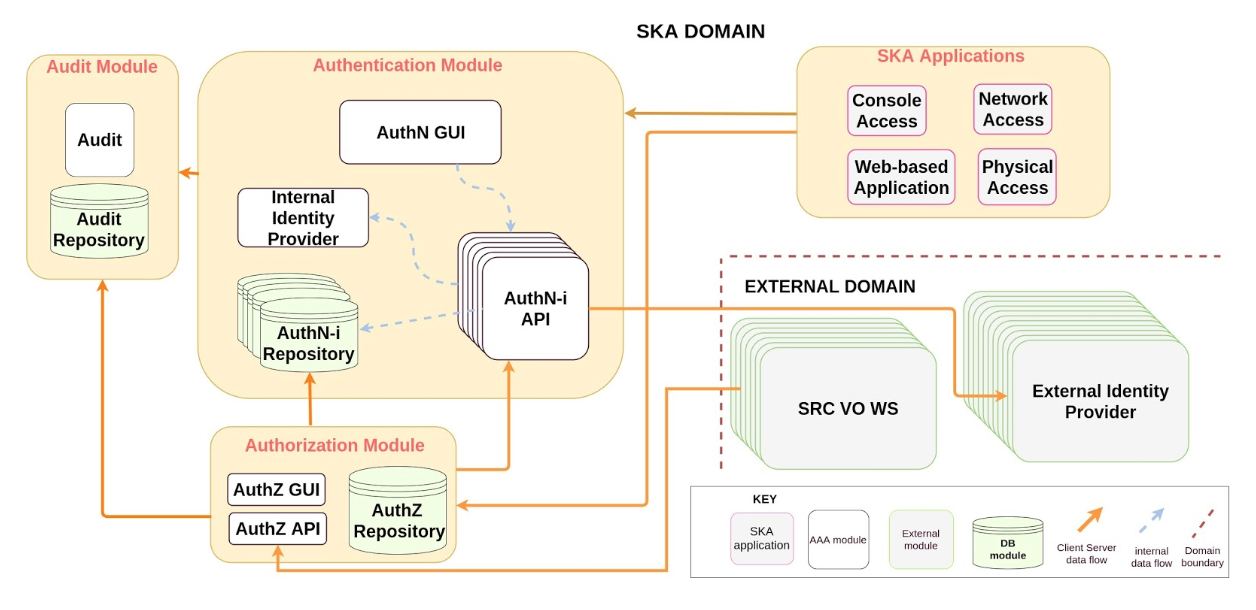
\includegraphics[width=0.7\columnwidth]{ska-domain.png}
  \caption{The SKA Domain}
  \label{fig:ska-domain}
\end{figure}

\begin{figure}[ht!]
  \centering
  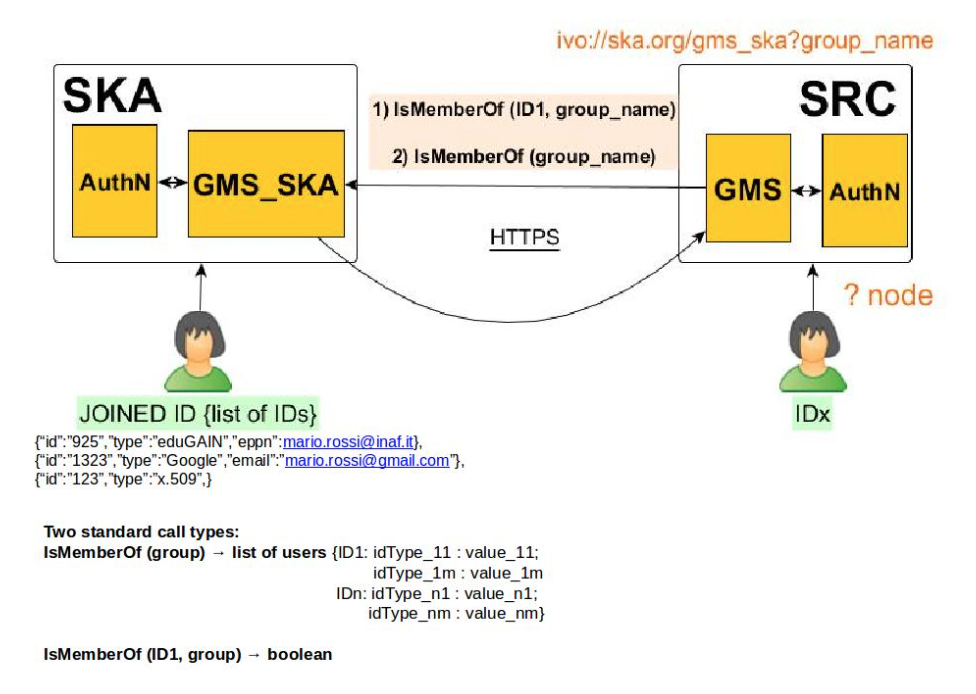
\includegraphics[width=0.7\columnwidth]{ska-auth.png}
  \caption{Mechanism for the authorisation interoperability}
  \label{fig:ska-auth}
\end{figure}

The authorisation sharing of information is protected via a trusted connection between the data centers. The strategy currently adopted for the trusted connection is to use the credential delegation protocol (a proxy certificate encapsulating a user certificate). A good choice could be to include more than one solution, so for example include also the Kerberos tickets and the exchange of private-public keys or a JSON array with the user attributes. The AAA system is suited with web based interfaces in order to allow registration and management of user credentials as well as administrative interfaces for supporting the activities of attributes maintenance and updates. The grouping management system can be reached both via REST calls and user interfaces in order to delegate as much as possible (and compatible with the SKA policy) the management of groups membership to the user that creates the group. A working and open instance could be found at https://sso.ia2.inaf.it.

\subsection{Virtual Atomic and Molecular Data Centre}
The Virtual Atomic and Molecular Data Centre is a consortium of Institutes and Research Institutions that share a common political and technical framework for the distribution and curation of atomic and molecular data: VAMDC aims to provide the international research community with access to provide A\&M data providers and compilers with a large dissemination platform for their work.
 
The political framework relies on rules of collaboration and organisation that are described in a Memorandum of Understanding.
 
The VAMDC Consortium technical framework relies on the use of the e-science VAMDC infrastructure that provides the international research community with access to a broad range of atomic and molecular (A\&M) data.
 
\textbf{Technical overview}
The e-Infrastructure federates \~41 heterogeneous atomic and molecular databases in an interoperable way: VAMDC provides a middleware, called Node Software, for transforming an autonomous database into a VAMDC node. Each node understands queries submitted with a given standard grammar\cite{vamdc-standards} and provides result formatted using the XSAMS standard (XML schema for Atoms, Molecules and Solids\cite{vamdc-ref}.  Each VAMDC node is registered into registries (a sort of yellow-pages of all the available services). When a user submit a query to VAMDC, this is dispatched to all the available services and the gathered result returned to the user. VAMDC is a distributed setting, with single point of access available\cite{vamdc-home} but no central management of the data or the infrastructure.
 
\textbf{Needs and requirement for Authentication, Authorisation and Accounting}
Atomic and Molecular data are crucial for several civilian and scientific uses. But they are also crucial for military purpose. As a consequence, some data may not be shared publicly with the community and their access may be open only possible for a selected set of users. For other categories of data, less confidential but potentially useful for military applications, VAMDC would like to track the origin and identity of the users.

An Authorisation, Authentication and Accounting strategy is very important for the VAMDC infrastructure.  Moreover, this is asked by our institute for measuring the impact of the VAMDC activity. The AAA strategy is fully discussed in the VAMDC RoadMap.  The main elements to retain are the following:
Since VAMDC
\begin{itemize}
\item do not want to handle the issue of passwords, registration/cancellation of users and
\item want to prevent a user who already has dozens of accounts (web mails, institutional IDs, social networks, etc.) to create a new specific one,
\end{itemize}
delegation of authorisation and usage of proxies are good technical solutions for meeting our needs.
 
The authentication, based on a mechanism of delegation, could be implemented on the VAMDC portal, for submitting queries and accessing data. However, since the VAMDC infrastructure is composed of autonomous nodes a shrewd and experienced user could bypass the authentication step: by using the standard query language, he/she could submit the queries and retrieve the data, directly from each node.

Therefore, some authentication mechanism must operate at each data node or other service that applies authorisation checks. The software and libraries providing access to data should implement the mechanism for the delegation of authentication, using the libraries provided by the retained mechanism of delegation: when a user authenticates, they will get information about its membership to the different existing virtual groups. This information will be passed to each VAMDC node, while performing the requests.

Authorised privileges for access data fall into two classes: access to specific, private records in the database; or improved access to the database as a whole, such as the ability to retrieve larger data-extracts. Node operators who opt to restrict access are free to set the specific authorisation rules. The identities authenticated at the nodes would typically be for user groups rather than individual users. The authorisation should be planned accordingly. If a node specifically needs to authorise individuals, then single-user ``groups" could be defined.
In the most basic version of accounting, we may compile macro-statistics for knowing (for each database node composing the VAMDC infrastructure):
\begin{itemize}
\item The amount of data extracted as a function of time (monthly and weekly scale)
\item The percentage of availability.
\item The specific tools/programs used for extracting data
\end{itemize}
At the present stage VAMDC has not implemented its AAA strategy since we are waiting a large consensus of the Data Sharing community on which solution retain for delegation of authentication.


\end{document}